% File: diploma.tex

\documentclass[
    14pt,
    specialist,
    candidate, % document type
    subf, % use and configure subfig package for nested figure numbering
    href,
    dotsinheaders=false
]{disser}

\hypersetup{colorlinks=false} % Configure hyperref loaded by disser class

% Кодировка и язык
\usepackage[T2A]{fontenc} % поддержка кириллицы
\usepackage[utf8]{inputenc} % кодировка исходного текста
\usepackage[english,russian]{babel} % переключение языков

% Геометрия страницы и графика
\usepackage[a4paper, mag=1000, left=3cm, right=1.5cm, top=2cm, bottom=2cm, headsep=0.7cm, footskip=1cm]{geometry}
\usepackage{graphicx} % подключение графики
\usepackage{pdfpages} % вставка pdf-страниц

% Таблицы
\usepackage{array} % расширенные возможности для работы с таблицами
\usepackage{tabularx} % автоматический подбор ширины столбцов
\usepackage{dcolumn} % выравнивание чисел по разделителю

% Математика
\usepackage{bm} % полужирное начертание для математических символов
\usepackage{amsmath} % дополнительные математические возможности
\usepackage{amssymb} % дополнительные математические символы
\usepackage{times}

% Библиография и ссылки
\usepackage{cite} % поддержка цитирования
% \usepackage[colorlinks=false]{hyperref} % Removed - loaded by 'href' class option
% \urlstyle{same}
% \renewcommand{\UrlFont}{\rmdefault}

% Прочее
\usepackage{color} % работа с цветом
\usepackage{epstopdf} % конвертация eps в pdf
\usepackage{multirow} % объединение ячеек таблиц по вертикали
\usepackage{afterpage} % вставка материала после текущей страницы
\usepackage{indentfirst} % отступ в первом абзаце раздела
\usepackage[font={normal}]{caption} % настройка подписей к рисункам и таблицам
\usepackage[onehalfspacing]{setspace} % полуторный интервал
\usepackage{fancyhdr} % установка колонтитулов
\usepackage{paratype} % моноширинный кириллический шрифт
\usepackage{listings} % поддержка вставки исходного кода
% \usepackage{newtxtext}
% \usepackage{newtxmath}
\usepackage{enumitem} % для настройки списков

% % Установка шрифта Times New Roman
\renewcommand{\rmdefault}{ftm}

% Установка абзацного отступа 1.25 см
\setlength{\parindent}{1.25cm}

% Убрать дополнительный интервал между абзацами одного стиля
\setlength{\parskip}{0pt}

% Настройка списков
\setlist{nosep} % убираем дополнительные отступы в списках
\setlist[itemize,1]{label={\textbullet}} % первый уровень маркированного списка
\setlist[itemize,2]{label={\textendash}} % второй уровень маркированного списка
\setlist[enumerate,2]{label={\alph{)}.}} % второй уровень нумерованного списка
\setlist[enumerate,1]{label={\arabic*.}, leftmargin=1.25cm, labelwidth=1cm, labelsep=0.25cm}

% Настройка стиля страницы
\pagestyle{fancy}      % Использование стиля "fancy" для оформления страниц
\fancyhf{}              % Очистка текущих значений колонтитулов
\fancyfoot[C]{\thepage} % Установка номера страницы в нижнем колонтитуле по центру
\renewcommand{\headrulewidth}{0pt} % Удаление разделительной линии в верхнем колонтитуле


% Настройка подписей к таблицам и рисункам
\captionsetup[table]{position=above, justification=raggedright, singlelinecheck=false, format=plain, labelformat=simple, labelsep=endash}
\captionsetup[figure]{position=below, justification=centering, singlelinecheck=true, format=plain, labelformat=simple, labelsep=endash}

% Настройка шрифта в таблицах
\let\oldtabular\tabular
\let\endoldtabular\endtabular
\renewenvironment{tabular}{\small\oldtabular}{\endoldtabular}

\makeatletter

% Define tab command for consistent spacing
\newcommand\tab[1][1.25cm]{\hspace*{#1}}

% Fix TOC to include dots between titles and page numbers
\renewcommand\@dotsep{4.5}
\renewcommand\tocpostthepart{\@postskip}
\renewcommand\tocpostthechapter{\@postskip}
\renewcommand\tocpostthesection{\@postskip}
\renewcommand\tocpostthesubsection{\@postskip}
\renewcommand\tocpostthesubsubsection{\@postskip}
\renewcommand\tocposttheparagraph{\@postskip}
\renewcommand\tocpostthesubparagraph{\@postskip}
% \renewcommand{\UrlFont}{\normalfont}

% Redefine TOC entry commands to use 14pt font and include dots
\renewcommand*\l@chapter[2]{%
  \ifnum \c@tocdepth >\m@ne
    % \vskip 1.0em \@plus\p@
    \setlength\@tempdima{2em}%
    \begingroup
    \parindent \z@ \rightskip \@pnumwidth
    \parfillskip -\@pnumwidth
    % \leavevmode \normalsize\bfseries\fontsize{14}{16}\selectfont
    \hskip -\leftskip
    #1\nobreak\leaders\hbox{\normalfont$\m@th\mkern \@dotsep mu\hbox{.}\mkern \@dotsep mu$}\hfill\nobreak\hb@xt@\@pnumwidth{\hss #2}\par
    \penalty\@highpenalty
    \endgroup
  \fi}

\renewcommand*\l@section[2]{%
  \ifnum \c@tocdepth >\z@
    % \vskip 1em \@plus\p@
    \setlength\@tempdima{2em}%
    \begingroup
    \parindent \z@ \rightskip \@pnumwidth
    \parfillskip -\@pnumwidth
    % \leavevmode \normalsize\fontsize{14}{16}\selectfont
    \hskip -\leftskip
    #1\nobreak\leaders\hbox{\normalfont$\m@th\mkern \@dotsep mu\hbox{.}\mkern \@dotsep mu$}\hfill\nobreak\hb@xt@\@pnumwidth{\hss #2}\par
    \penalty\@highpenalty
    \endgroup
  \fi}

\renewcommand*\l@subsection[2]{%
  \ifnum \c@tocdepth >\@ne
    % \vskip 1em \@plus\p@
    \setlength\@tempdima{3em}%
    \begingroup
    \parindent \z@ \rightskip \@pnumwidth
    \parfillskip -\@pnumwidth
    \leavevmode \normalsize\fontsize{14}{16}\selectfont
    \hskip -\leftskip
    #1\nobreak\leaders\hbox{\normalfont$\m@th\mkern \@dotsep mu\hbox{.}\mkern \@dotsep mu$}\hfill\nobreak\hb@xt@\@pnumwidth{\hss #2}\par
    \penalty\@highpenalty
    \endgroup
  \fi}

% Add a flag to track if we're immediately after a chapter
\newif\if@afterchapter
\@afterchapterfalse

% Make chapter titles bold and centered with proper anchoring - ALL CAPS for first level
\newcommand{\mychapter}[1]{%
  \newpage
  \refstepcounter{chapter}% Move counter increment inside the command
  \hypertarget{chap:\thechapter}{}% Create unique anchor
  \begin{center}
    \textbf{\MakeUppercase{\thechapter\space #1}}
  \end{center}
  % Reduce space between number and title in TOC by using less space or negative space
  \addcontentsline{toc}{chapter}{\texorpdfstring{\thechapter\hspace{0.3em}#1}{Chapter \thechapter}}% Reduced space
  \@afterchaptertrue % Set flag after chapter
}

% Special command for unnumbered chapters (like INTRODUCTION, CONCLUSION)
\newcommand{\myunnumberedchapter}[1]{%
  \newpage
  \hypertarget{chap:#1}{}% Create unique anchor
  \begin{center}
    \textbf{\MakeUppercase{#1}}
  \end{center}
  \addcontentsline{toc}{chapter}{\texorpdfstring{#1}{#1}}% Add optional PDF string
}

\newcommand{\mysection}[1]{%
  \ifnum\value{section}>0
  \vspace{1em}
  \fi
  \refstepcounter{section}
  \hypertarget{sec:\thechapter.\thesection}{}% Create unique anchor
  \textbf{\thesection\space #1}
  % Reduce space between number and title in TOC
  \addcontentsline{toc}{section}{\texorpdfstring{\thesection\hspace{2em}#1}{Section \thesection}}% Reduced space
}

\newcommand{\mysubsection}[1]{%
  \refstepcounter{subsection}
  \hypertarget{subsec:\thechapter.\thesection.\thesubsection}{}
  \textbf{\thesubsection\space #1}
  % Reduce space between number and title in TOC
  \addcontentsline{toc}{subsection}{\texorpdfstring{\thesubsection\hspace{2em}#1}{Subsection \thesubsection}}
}

\renewcommand{\thechapter}{\arabic{chapter}}

% Define appendix format with Cyrillic letters
\newcommand{\startappendix}{%
  \setcounter{chapter}{0}%
  \renewcommand{\thechapter}{\CYRA\cyrillictext}%
  \renewcommand{\thesection}{\thechapter.\arabic{section}}%
  \renewcommand{\thesubsection}{\thechapter.\arabic{section}.\arabic{subsection}}%
  \renewcommand{\thetable}{\thechapter.\arabic{table}}%
  \renewcommand{\thefigure}{\thechapter.\arabic{figure}}%
}

\makeatother

\AtBeginDocument{\onehalfspacing}

% Настройка листингов кода (перед \begin{document})
\lstset{
    basicstyle=\normalsize\ttfamily,        % базовый шрифт нормального размера
    numberstyle=\normalsize\ttfamily,       % шрифт нумерации того же размера
    numbers=left,                           % нумерация строк слева
    numbersep=6pt,                          % отступ номеров от кода
    frame=single,                           % единая рамка
    framerule=0.8pt,                        % толщина рамки
    framexleftmargin=17pt,                  % рамка захватывает номера строк
    xleftmargin=17pt,                       % отступ слева для выравнивания
    captionpos=t,                           % заголовок сверху
    breaklines=true,                        % перенос длинных строк
    showstringspaces=false,                 % не показывать пробелы в строках
    resetmargins=true,                      % сброс полей
    aboveskip=10pt,                         % отступ сверху
    belowskip=10pt                          % отступ снизу
}

% Переопределение названий для листингов
\renewcommand{\lstlistingname}{Листинг}

% Настройка подписей к листингам через caption
\captionsetup[lstlisting]{
    singlelinecheck=false,
    justification=raggedright,
    format=plain,
    labelformat=simple,
    labelsep=endash
}

% Настройка формата номеров листингов
\makeatletter
\AtBeginDocument{
  % Переопределение формата номера листинга
  \renewcommand{\thelstlisting}{\arabic{lstlisting}}
}
\makeatother

\begin{document}

\sloppy


\includepdf[pages={1-5}]{./assets/TitlePage.pdf}

\renewcommand{\contentsname}{\centerline{\normalsize\bfseries\centerline{\textbf{\MakeUppercase{СОДЕРЖАНИЕ}}}}}
\setcounter{tocdepth}{1}

\tableofcontents

\myunnumberedchapter{ВВЕДЕНИЕ}

В современной инновационной экономике проблема эффективного распределения ресурсов на ранних стадиях развития проектов остается одной из наиболее остро стоящих. Существующие механизмы финансирования, от традиционного венчурного капитала до акселерационных программ, зачастую не способны ответить на вызовы с которыми сталкиваются начинающие проекты. Неравномерное распределение информации, субъективизм в оценках, ошибки на этапе проверки гипотез. Это порождает значительные барьеры, особенно для тех, кто стремится быстро и с минимальными издержками валидировать идеи, не попадая в зависимость от длительных циклов отбора или ограниченных грантовых программ.

На этом фоне возникает объективная потребность в создании альтернативной системы, обеспечивающей более прозрачную, масштабируемую модель распределения инвестиционных ресурсов. В настоящей работе рассматривается подход к построению такой системы на основе блокчейн-технологий и алгоритмов объективной оценки, способной выполнять функции рыночной валидации идей. Предлагаемый механизм устраняет ряд фундаментальных ограничений традиционных моделей: снижает асимметрию информации, минимизирует субъективность принятия решений.

Актуальность исследования определяется необходимостью разработки эффективного и воспроизводимого способа взаимодействия между стартапами и инвесторами на начальных стадиях, способного ускорить трансформацию идей в реальные проекты.

Целью данной работы является формализация нейросетевого механизма распределения ресурсов с последующим его масштабированием в архитектуре децентрализованного приложения для инвестиционной оценки стартапов.

Для достижения поставленной цели в работе решаются следующие задачи:
\begin{enumerate}
  \item Проанализировать предметную область и актуальность.
  \item Рассмотреть аналоги и целевую аудиторию.
  \item Изучить теоретические основы распределения ресурсов.
  \item Обобщить теоретическую модель.
  \item Составить экономическое обоснование для применения в предметной области.
  \item Применить модель в рамках оптимизационной стратегии.
  \item Описать бизнес-процессы в системе.
  \item Спроектировать архитектуру приложения.
  \item Разработать ядро системы.
  \item Разработать серверную часть приложения.
  \item Разработать клиентскую часть приложения.
  \item Проанализировать результаты и перспективы дальнейшего внедрения.
\end{enumerate}

Предметом исследования являются механизмы распределения ресурсов и оценки инновационных проектов на ранних стадиях, основанные на технологиях блокчейн и искусственного интеллекта. Объектом исследования выступает процесс инвестирования в ранние стадии инновационных проектов.

Практическая значимость работы заключается в создании новой парадигмы инвестирования, которая позволит преодолеть структурные ограничения существующих механизмов и обеспечить более эффективное распределение капитала для инновационных проектов. Это может способствовать ускорению технологического развития, созданию новых рабочих мест и повышению глобальной конкурентоспособности экономики.

% ## 1
\mychapter{АНАЛИТИЧЕСКИЙ ОБЗОР}

% ### 1.1
\mysection{Анализ предметной области}

Рынок инвестиций в стартапы на ранних стадиях представляет собой сложную и многогранную экосистему, в которой участвуют разнообразные субъекты – от основателей и индивидуальных инвесторов до венчурных фондов и корпоративных акселераторов. Такая экосистема характеризуется высокой степенью неопределенности и информационной асимметрией, что приводит к появлению структурных проблем, негативно влияющих на эффективность распределения ресурсов.

Анализ текущей динамики венчурного рынка также демонстрирует институционализацию стартапов как полноценного элемента современной экономики. Согласно данным Global Innovation Index 2024 \cite{gii2024}, доля венчурных инвестиций по отношению к ВВП уверенно растёт не только в странах с высоким уровнем дохода, но и в странах со средним уровнем развития, что показано на рисунке~\ref{fig:vc-gdp-share}. Это свидетельствует о снижении барьеров для вхождения в стартап-экосистему и подтверждает всё более системную роль стартапов в экономическом росте и распределении инновационного капитала.

\begin{figure}[h]
  \centering
  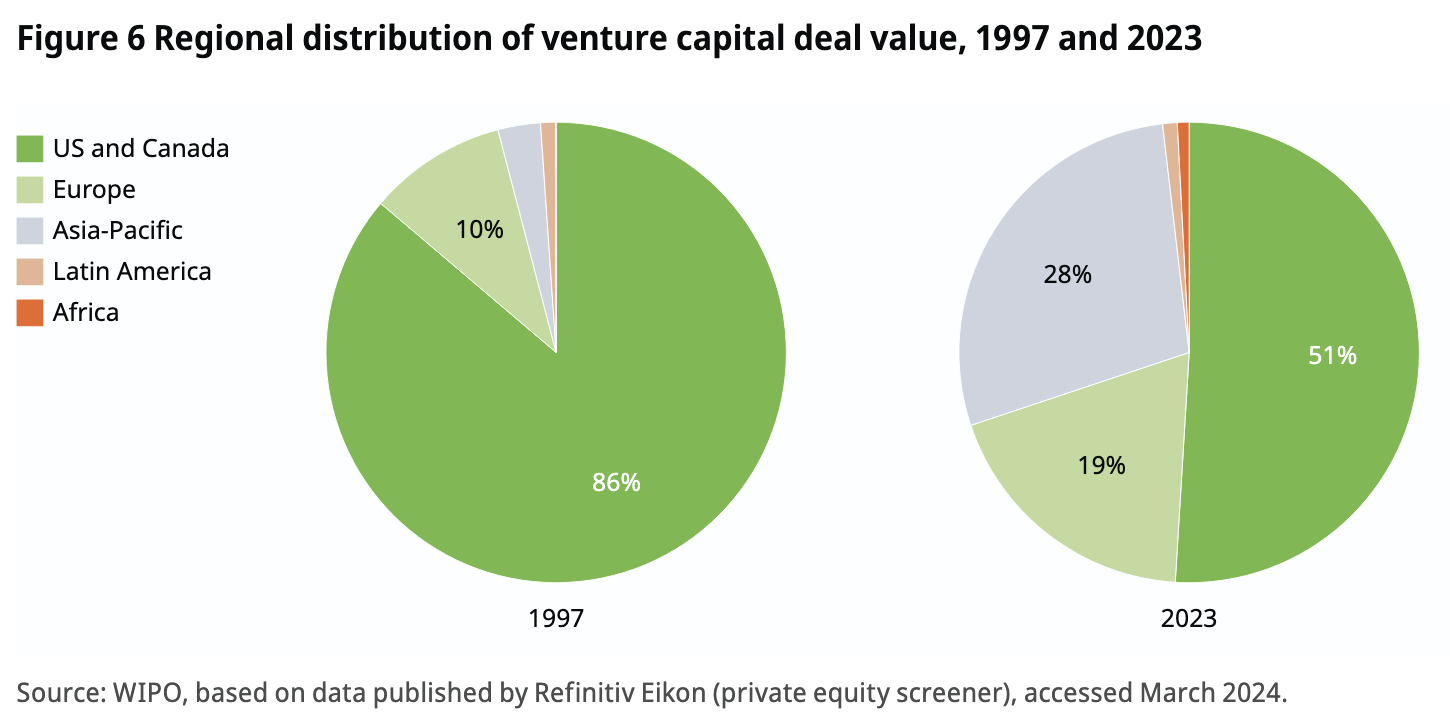
\includegraphics[width=0.75\textwidth]{assets/vc-gdp-share.png}
  \caption{Доля венчурных инвестиций по отношению к ВВП в странах с различным уровнем дохода. Источник: Global Innovation Index 2024~\cite{gii2024}.}
  \label{fig:vc-gdp-share}
\end{figure}

Это приводит к тому, что перспективные проекты с несовершенной маркетинговой стратегией или без связей остаются незамеченными. За счет узкого охвата потенциальных инвесторов субъективность оценки, основанная на личных впечатлениях или косвенных сигналах (например, репутации основателя) усиливает предвзятость.

Эта асимметрия порождает систематическую субъективность в оценках: решения о финансировании по большей части принимаются на основе неформализованных критериев и «интуитивных» сигналов, а не объективных метрик. Вследствие этого капитал концентрируется вокруг ограниченного круга проектов, которые получают повышенное внимание за счёт лучших контактов или более ярких презентаций, тогда как остальные идеи, не обладающие значительной социальной поддержкой, оказываются без шансов на развитие.

Кроме того, отсутствие встроенных механизмов ликвидности создаёт экономический разрыв между стадиями запуска и выхода из проекта: инвесторы вынуждены искать внешние площадки или договариваться о выкупе долей, что замедляет оборот капитала и увеличивает транзакционные издержки. Наконец, устойчивость инновационной экосистемы подрывает эффект «инвестиционных каскадов», когда решения небольшого круга лидирующих инвесторов задают тренд для всего рынка, нивелируя разнообразие взглядов и препятствуя объективной проверке гипотез.

Эти вызовы приводят к неоптимальному распределению капитала, замедляя развитие инновационной экосистемы. Именно в этой среде, где традиционные финансовые инструменты оказываются неприспособленными к особенностям распределённых сетей, появляется острая потребность в механизмах, способных объективно агрегировать коллективную экспертизу, автоматически устанавливать ценность проектов и обеспечивать устойчивую ликвидность.

Анализ предметной области инвестиций в стартапы ранних стадий демонстрирует, что на этом этапе стоимость проектов формируется не реальными денежными потоками, а ожиданиями и верой участников экосистемы. Отсутствие стабильных финансовых показателей заставляет инвесторов полагаться на фрагментарные данные — результаты первых прототипов, отзывы пользователей, а порой и просто репутацию команды — что приводит к существенной информационной асимметрии.

% ### 1.2
\mysection{Определение актуальности}

Основатели стартапов сталкиваются с необходимостью быстрой проверки своих идей на жизнеспособность.

Традиционные механизмы, такие как венчурный капитал или акселерационные программы, часто требуют длительных циклов отбора, раскрытия критически важной информации и подчинения строгим условиям, что создает барьеры для быстрой рыночной валидации. В то же время инвесторы, ориентированные на диверсификацию портфеля за счет перспективных, но еще не оформившихся инициатив, нуждаются в надежных инструментах для оценки широкого спектра проектов и оптимального распределения капитала. Текущие подходы, основанные на дискретных инвестиционных раундах, ограничивают выборку доступных стартапов и усиливают монополию крупных игроков, оставляя множество потенциально прорывных идей без поддержки.

Одной из ключевых проблем является информационная асимметрия между основателями стартапов и потенциальными инвесторами. Основатели обладают глубоким пониманием своих проектов, однако при необходимости привлечения инвестиций вынуждены подстраивать это понимание под маркетинговый контекст. В свою очередь, инвесторы ограничены в доступе к полной информации о проекте и его перспективах, что затрудняет объективную оценку и вынуждает опираться на косвенные сигналы, такие как образование и опыт основателей.

Особенно ярко это проявляется в блокчейн стартапах, ведь им необходим пул ликвидности для обеспечения бесперебойной торговли, стабильности цен и доверия пользователей к их токену или платформе. Пул ликвидности — это резерв цифровых активов, хранящийся в блокчейне и предназначенный для автоматического обмена токенов по заранее установленным правилам без участия посредников.

Обеспечение достаточного уровня ликвидности является фундаментальным условием эффективного функционирования блокчейн-стартапов, поскольку именно она обеспечивает непрерывность торговых операций, минимизирует проскальзывание и способствует поддержанию стабильности ценового уровня токена. Глубокая ликвидность выступает индикатором здоровой экосистемы, привлекает трейдеров, предпочитающих площадки с низкой ценовой волатильностью, и формирует доверие инвесторов к проекту, что, в свою очередь, усиливает сетевой эффект и стимулирует дальнейшее расширение пользовательской базы. При недостаточном объёме ликвидности даже незначительные сделки способны вызвать существенные колебания цены, создавая угрозу массового оттока участников и повышая риски ценовых манипуляций со стороны крупных держателей.

Достижение и поддержание необходимого уровня ликвидности осуществляется с помощью ряда финансовых и организационных подходов. В первую очередь, для быстрого привлечения средств используются программы, которые поощряют участников сообщества размещать свои активы в пулах за вознаграждение. Другим распространённым способом является первичное размещение токенов на децентрализованных биржах, позволяющее одновременно привлечь инвестиции и сформировать начальный резерв активов для торговли.

Также применяется подход, при котором сам проект выпускает специальные облигации или аналогичные финансовые инструменты, чтобы напрямую владеть ликвидностью, избегая зависимости от временных внешних вложений.

Ещё одним вариантом является привлечение профессиональных организаций, специализирующихся на создании ликвидности, что позволяет обеспечить необходимый объём активов для торговли без значительных собственных расходов проекта.

Дополнительно используется размещение токенов на крупных централизованных биржах при поддержке профессиональных участников рынка, что расширяет круг потенциальных инвесторов и повышает популярность проекта.

Наконец, важным методом выступает применение автоматизированных алгоритмов, которые обеспечивают непрерывное формирование цен и постоянный доступ участников к торговле, снижая при этом резкие колебания цены и увеличивая доверие пользователей к платформе.

Комплекс этих проблем создаёт существенные барьеры для эффективного функционирования рынка инвестиций в ранние стадии, приводя к неоптимальному распределению капитала, когда перспективные проекты остаются без необходимой поддержки, а проекты с меньшим потенциалом, но лучшей презентацией или более сильными социальными связями, получают непропорционально большие инвестиции, что в конечном итоге снижает эффективность инновационной экосистемы и замедляет технологический прогресс.

% ### 1.3
\mysection{Описание целевой аудитории}

Портрет целевой аудитории платформы включает в себя две ключевые группы: основателей стартапов и инвесторы, ориентированных на высокорисковые, но потенциально доходные вложения.

Первыя группу составляют преимущественно молодые люди от 20 до 35 лет. Они нуждаются в доступе к капиталу, который должен основываться на объективной оценке потенциала идеи, а не на субъективных факторах, таких как опыт, образование или социальные связи, что подтверждается тем, Отсутствие качественной обратной связи представляет существенное препятствие для развития их проектов. Они стремятся минимизировать затраты времени и ресурсов на привлечение инвестиций, что особенно актуально, учитывая, что процесс привлечения посевного финансирования в среднем занимает от шести до девяти месяцев.

Вторую группу составляют инвесторы ранних стадий, для которых важным является обеспечение доступа к качественному потоку сделок с высоким потенциалом. Помимо этого, инвесторам необходимы объективные данные для оценки потенциала проектов в условиях ограниченного объёма информации; Наконец, инвесторы стремятся к диверсификации инвестиционного портфеля, предпочитая инвестировать в большое кол-во проектов, что позволяет распределить риски, несмотря на ограничения, связанные с оценкой большого количества проектов.

Учитывая, что обе группы действуют в условиях высокой неопределённости и переизбытка информации, внимание становится дефицитным ресурсом. Рынок инноваций и венчурного капитала всё чаще функционирует по законам экономики внимания, где первичную роль играет не только содержание, но и форма подачи. Визуально привлекательный, яркий, интуитивно понятный интерфейс становится не просто инструментом взаимодействия с продуктом, а критическим фактором захвата и удержания пользователя, особенно в условиях растущей конкуренции за внимание. Он способствует не только улучшению пользовательского опыта, но и формирует доверие к технологической и инновационной зрелости платформы.

Проведённый анализ целевой аудитории демонстрирует, что, несмотря на различия в потребностях, стейкхолдеры заинтересованы в создании более эффективной, объективной и прозрачной системы оценки и финансирования инновационных проектов на ранних стадиях. В этом контексте яркий, современный и эмоционально вовлекающий интерфейс представляет собой не эстетическую деталь, а стратегически важный инструмент, способствующий расширению аудитории, повышению вовлечённости пользователей и достижению маркетинговых целей на конкурентном рынке.

% ### 1.4
\mysection{Обзор существующих решений}

В современной экосистеме инвестирования применяются различные подходы, каждый из которых частично решает обозначенные проблемы, но не способен обеспечить

Основные практики привлечения инвестиций включают традиционное венчурное финансирование, участие в акселерационных программах, краудфандинг.

Венчурные фонды и инвесторы представляют собой наиболее распространённый механизм финансирования ранних стадий, основанный на личных встречах, презентациях и субъективной оценке потенциала проектов и команд. Преимущества данного подхода заключаются в наличии доступа к экспертной поддержке и менторству, возможности установления долгосрочных отношений между основателями и инвесторами, гибкости в структурировании сделок и условия инвестирования, а также наличии широкой сети контактов, которую инвесторы могут предоставить. Однако существенные ограничения этого механизма проявляются в высокой степени субъективности и предвзятости при оценке проектов, Согласно \cite{imbierowicz2024peer}, оценки стартапов на ранних стадиях часто опираются не на бизнес-фундамент, а на ориентиры из недавних сделок в смежных сегментах, что приводит к эффекту переоценки и рыночной нестабильности. Дополнительно, зависимость от социальных связей и репутации, а также необходимость полного раскрытия идеи, создающая риск для интеллектуальной собственности и географическая концентрация венчурных инвестиций, ограничивающая доступ к капиталу для основателей из других регионов, существенно снижают эффективность данного подхода.

Акселераторы и стартап-инкубаторы, такие как Y Combinator, Techstars, AngelList, предлагают структурированные программы поддержки стартапов, объединяющие менторство, образовательные компоненты и доступ к инвесторам. Структурированный процесс отбора и поддержки проектов создаёт чёткие рамки для развития, что особенно важно для неопытных основателей \cite{thiel2014zero}, а доступ к обширным сетям контактов и экспертизе ускоряет валидацию идей и выход на рынок. При этом частичная автоматизация инвестиционных процессов снижает транзакционные издержки, а стандартизация документации упрощает юридические аспекты финансирования. Главной проблемой здесь является высокая конкуренция за места в ведущих программах (например, Y Combinator принимает менее 1\% заявителей \cite{yc_acceptance_rate}) значительно снижает шансы на участие и отсеивает потенциально хорошие идеи. Также, географические ограничения продолжают оставаться барьером для основателей, расположенных вне основных инновационных хабов.

Альтернативными механизмами являются платформы краудфандинга, которые способствуют демократизации доступа к инвестициям, позволяя привлекать финансирование без зависимости от традиционных связей, а также обеспечивают валидацию идеи через прямой отклик потенциальных пользователей. Такие подходы также способствуют созданию сообщества вокруг проекта на ранних стадиях, однако часто решения о финансировании принимаются исключительно за счет маркетингово продвижения, что может приводить к поддержке коммерчески нежизнеспособных проектов. По данным отчёта KingsCrowd \cite{kc2024}, несмотря на постепенное снижение общего объёма инвестиций в рамках краудфандинга (рис.~\ref{fig:regcf-investments}), количество инвестиционных сделок демонстрирует устойчивый рост (рисунок ~\ref{fig:crowd-funding}). Это указывает на рост популярности малых инвестиционных раундов.

\begin{figure}[h]
  \centering
  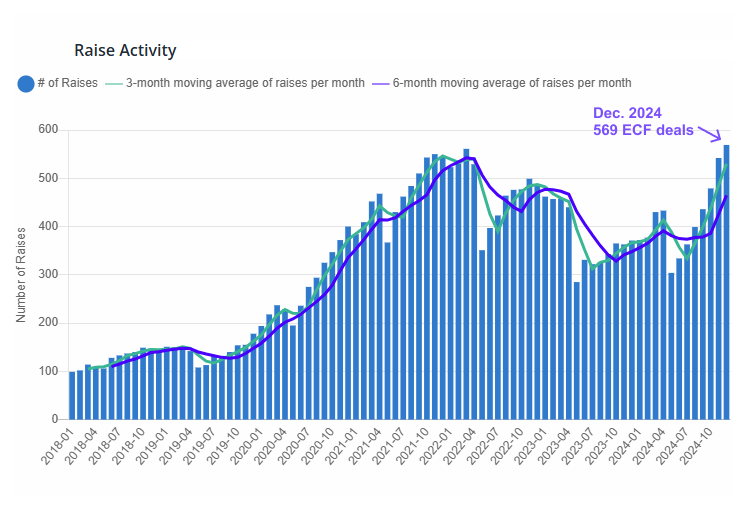
\includegraphics[width=0.9\textwidth]{./assets/crowd-funding.png}
  \caption{Рост числа инвестиций}
  \label{fig:crowd-funding}
\end{figure}

Сравнительный анализ эффективности существующих подходов показывает, что ни один не способен обеспечить одновременно, объективную оценку проектов и оптимальное распределение капитала. Стоит отметить, что сильной стороной традиционных подходов является их структурированность и наличие экспертной поддержки, особенно в случае венчурных фондов и акселераторов, где стартапы получают доступ к опыту и связям \cite{lange2024angels}. Однако слабые стороны этих механизмов существенно ограничивают возможности их масштабирования.

% ### 1.5
\mysection{Вывод по первой главе}

Таким образом, проведенный анализ указывает на необходимость создания комплексного механизма, который бы одновременно обеспечивал объективную оценку проектов и оптимальное распределение капитала с учётом как объёма инвестиций, так и широты поддержки аудиторией.

% Глава 2
% ###############################################################
\mychapter{ТЕОРЕТИЧЕСКИЕ ОСНОВЫ РАСПРЕДЕЛЕНИЯ РЕСУРСОВ}


% ### 2.1 Обзор проблематики
\mysection{Предметная область}

Вопрос распределения ограниченных ресурсов встречается во множестве областей: от найма сотрудников и распределения ролей в проекте до управления вычислительными мощностями и каналами связи. Несмотря на кажущуюся простоту локальных задач, универсальная платформа, способная учесть все требования и компромиссы, оказывается невозможной из-за многомерности критериев и конфликтующих интересов участников(Hurwicz, 1972). Вместо единого решения человечество выработало специализированные механизмы в разных контекстах, каждый из которых успешно справляется с узконаправленными задачами, но не гарантирует оптимальности в общей постановке проблемы.
в связи с реавлицией в цифровых финансах и нейросетях
\cite{vaswani2017attention}

% ## 2.2
\mysection{Экономические принципы}

Рынки - это, пожалуй, самая мощная распределенная система, которую когда-либо
создавало человечество. В отличие от искусственных конструкций, рынки никогда не создавались специально; скорее,
они спонтанно возникли из нашего фундаментального человеческого желания торговать.

Когда люди стремятся обменяться товарами или услугами, они естественным образом собираются в общих пространствах — физических
торговых площадках, кофейнях или цифровых форумах — и благодаря этим взаимодействиям создается важнейший технологический побочное явление: рыночная цена.

Первоначально отдельные обмены происходят в различных соотношениях, поскольку каждый участник ведет переговоры, основываясь на субъективных оценках. Однако по мере того, как на рынок выходит все больше участников, индивидуальные различия постепенно уменьшаются, и цены неизбежно приближаются к общему среднему показателю. Эта средняя цена становится мощным источником коллективного разума, воплощающим совокупность знаний и ожиданий всех участников рынка.

Интересно, что трейдеры исторически разрабатывали новые системы коммуникации для эффективной передачи рыночной информации. Каждая инновация - от открытых площадок для обсуждения до телеграфа и, в конечном счете, современного Интернета - расширяла возможности рынка по обработке и распространению информации, привнося в цену глубокий коллективный разум. Наблюдатели вскоре поняли, что эти рыночные цены содержат уникальную, ценную информацию, раскрывающую
скрытые истины и прогнозирующую будущие события.

Однако возникает естественный вопрос: почему никто не может использовать частную информацию с выгодой для себя?

Это ключевая особенность. Попытки торговать секретной информацией не ухудшают рынок, а, наоборот , повышают его достоверность. Каждая конфиденциальная сделка раскрывает скрытые знания , соответствующим образом корректируя цены, тем самым повышая точность и надежность
коллективных прогнозов рынка.

Это явление, наблюдаемое в таких случаях, как влияние погоды на фьючерсы на апельсины или коэффициенты ставок на спорт, позволяет прогнозировать цены, отражая не только текущее значение, но и будущие ожидания.

\begin{figure}[h]
  \centering
  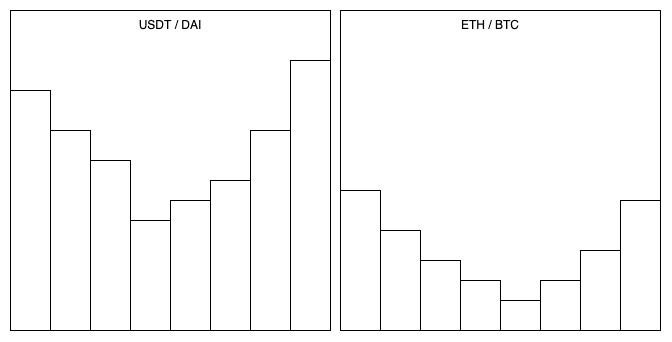
\includegraphics[width=0.9\textwidth]{./assets/limit-order.drawio.png}
  \caption{График глубины рынка для торговых пар с высокой и малой ликвидностью}
  \label{fig:limit-order}
\end{figure}

В конечном счете, объединение различных рыночных систем — традиционных, прогнозирующих и вычислительных - создает единый глобальный механизм. Такая интеграция повышает потенциал
коллективного разума, превращая разрозненную информацию в действенные идеи и решения. Такая взаимосвязанность превращает сотрудничество между людьми в масштабируемую интеллектуальную
экономическую машину, способную постоянно адаптироваться и развиваться, фактически становясь самым мощным вычислительным механизмом человечества.

\begin{figure}[h]
  \centering
  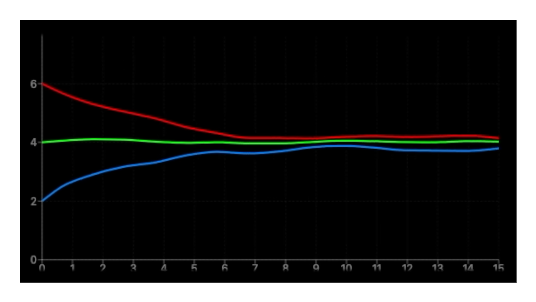
\includegraphics[width=0.9\textwidth]{./assets/one-price.png}
  \caption{Сходятся}
  \label{fig:limit-orders-2}
\end{figure}

% ## 2.3
\mysection{Сопоставление стратегий}

Это свойство рынка заставляет нас рассмотреть гипотетическую, но логичную последовательность действий: что, если бы мы полностью отказались от немедленных транзакций, сосредоточившись исключительно на ставках на результаты будущих событий? Такой рынок выражал бы скорее вероятности, чем ценности. Действительно, такие структуры уже существуют — они известны как рынки прогнозов — и в них заложен принципиально иной рыночный механизм. Эти рынки прогнозов дают вероятностные оценки, объединяя различные и даже противоречивые точки зрения для получения
удивительно точных прогнозов.

Критики могут возразить, что этими рынками можно манипулировать. Однако, если кто-то искренне верит, что рынками прогнозирования легко манипулировать, он неявно заявляет
о превосходстве личных знаний над совокупным пониманием бесчисленного количества участников — смелое утверждение.

И наоборот, если признать рынки прогнозирования надежными и правдивыми,
то при разработке децентрализованного приложения для оценки инвестиций возникает не менее провокационный вопрос: почему бы не доверить принятие важных решений непосредственно таким
рынкам?

Предел централизации (единоличный разум, ИИ)
Преимущества:
- Простая архитектура: один ИИ обрабатывает все решения.
- Быстрая реакция на входные данные.
- Подходит для небольших и менее критичных систем.
- Может эффективно использовать конфиденциальную информацию без публичного раскрытия.

Недостатки:
- Нет нейтральности: модель обучается на предвзятых данных, содержит скрытые предпочтения.
- Отсутствие прозрачности: даже при открытых весах сложно понять поведение модели.
- Сложность и непрозрачность: модель содержит десятки миллиардов бит информации — сравнимо с полной юридической системой США.
- Частые обновления: из-за быстрой эволюции ИИ «модель» фактически меняется каждые 3 месяца.
- Централизация власти: управляет тот, кто контролирует модель и её обновления.

Где каждый агент голосует ресурсами
Преимущества:
Недостатки:

Остальные модели (DAO, голосование, делегация) можно рассматривать как гибриды или переходные формы.

\begin{figure}[h]
  \centering
  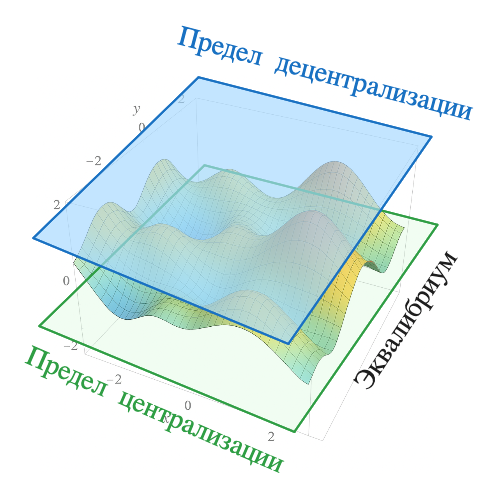
\includegraphics[width=0.5\textwidth]{./assets/de-centralization.png}
  \caption{Сравнение предел централизации и придела децентрализации}
  \label{fig:limit-orders}
\end{figure}

% ## 2.4
\mysection{Модель распределения ресурсов}

В системном виде распределение сводится к трём компонентам.

Во-первых, сеть агентов получает входные данные – частные знания, сигналы окружения и параметры правил игры.

Во-вторых, каждый агент применяет локальные правила (stake, голосование, покупка), формируя «выходные действия». В-третьих, через механизм согласования (консенсус), эти действия агрегируются в глобальное состояние, по которому затем все агенты синхронизируют новую итерацию.

[Рисунок 3: блок-диаграмма распределённой системы «вход – контроллер – выход»]

При этом внутри каждого агента может реализовываться аналогичная структура, образуя рекурсивно вложенную среду: на уровне мета-игры «правила игры» сами настраиваются (через AI-стирающую компоненту), а на нижних уровнях ведётся локальная оптимизация под заданные стимулы.

% ## 2.5
\mysection{Вывод по второй главе}

Из рассмотренного следует, что для построения эффективного механизма распределения ресурсов необходима архитектура, сочетающая в себе следующие свойства:
\begin{itemize}
  \item наличие «вычислительной» силы в виде локальных экспертиз;
  \item стимулы для добровольного участия в механике выигрыша или потерь;
  \item доверенный механизм согласования локальных решений в единую глобальную норму.
\end{itemize}
Такая система, обладает свойством адаптации к условиям среды, тем самым эффективно решая задачи динамического распределения ресурсов.

% #####################################################
% Глава 3
\mychapter{МАСШТАБИРОВАНИЕ МОДЕЛИ ИНВЕСТИЦИОННОЙ ОЦЕНКИ}
% #####################################################

% ## 3.1
\mysection{Формализация предметной области}

Рассмотрим множество проектов $P = \{p_1, p_2, \dots, p_n\}$, каждый из которых стремится привлечь определённый капитал $C_i$ для своего развития. Также рассмотрим множество агентов (пользователей системы) $A = \{a_1, a_2, \dots, a_m\}$, которые могут участвовать в финансировании проектов и получать токены пропорционально своим вкладам.

Каждый агент $a_j$ может вложить капитал $c_{ij}$ в проект $p_i$, получая взамен токены $t_{ij}$. Центральной задачей является оптимальное распределение ограниченного общего пула капитала $M$ таким образом, чтобы максимизировать общую полезность агентов и минимизировать возможность манипуляций. Для чистоты эксперимента рассматриваются только новые стартапы, лишённые скрытых параметров и маркетинговых кампаний, что позволяет объективно и точно прогнозировать их успех.

% ## 3.2
\mysection{Экономическое обоснование}

Общеизвестная теорема Кондорсе о жюри \cite{condorcet1785essay} утверждает, что если каждый агент делает правильные прогнозы с вероятностью чуть выше 50\%, то точность коллективного решения экспоненциально растёт с увеличением количества агентов.

Индивидуальный инвестор ограничен собственной неполной информацией и когнитивными искажениями. Однако группа агентов, действующая без скоординированных манипуляций, эффективно агрегирует частичную информацию, формируя более точное представление о перспективности стартапа.


% Экспоненциальный рост точности прогнозов согласно теореме Кондорсе.

Для обеспечения стимулов к честной игре и защиты от манипуляций, в системе реализован механизм Proof of Stake (PoS) \cite{king2012ppcoin},


Токенизацией через Augmented Bonding Curve (ABC) и механизмом Quadratic Funding (QF). Кривая ABC определяется формулой:
\[
  P(s) = \alpha \cdot s^\beta, \quad \beta = \frac{1}{1-r}, \quad r \in (0,1),
\]
где $s$ — текущее количество выпущенных токенов, $\alpha$ — масштабный коэффициент, а $r$ — резервный коэффициент. QF распределяет финансирование из общего пула на основе квадратичной функции индивидуальных вкладов:
\[
  M_i = \left(\sum_j \sqrt{c_{ij}}\right)^2,
\]
обеспечивая преимущество массовой поддержки над единичными крупными вкладами.

% Мллюстрацию механизма ABC+QF с примерами распределения финансирования.

% ## 3.3
\mysection{Оптимизационная стратегия}

Основной уязвимостью QF являются Sybil-атаки, устранение которых реализовано по аналогии с помощью меранизма proof of stake \cite{} создающим экономический барьер для многочисленных фейковых аккаунтов.

Почему нельзя обмануть систему? \cite{nakamoto2008bitcoin}

Согласно теории игр, описанный механизм приводит систему к динамическому равновесию Нэша \cite{nash1951non}, в котором ни одному агенту не выгодно отклоняться от честного поведения. Каждый агент ставит часть капитала (stake), рискуя им при оценке проекта. Если его прогноз согласуется с коллективным результатом, ставка возвращается с прибылью, иначе частично или полностью теряется. Таким образом, рациональный агент мотивирован действовать честно и использовать всю доступную ему информацию.

Дополнительно реализован механизм на основе Reinforcement Learning (RL), который адаптивно настраивает параметры токеномики (например, коэффициенты ABC и требования по ставкам), минимизируя возможности для манипуляций и усиливая стимулы к честной игре:
\[
  \pi^* = \arg\max_{\pi} \mathbb{E}\left[\sum_{t=0}^{\infty} \gamma^t R_t\right].
\]

\begin{figure}[h]
  \centering
  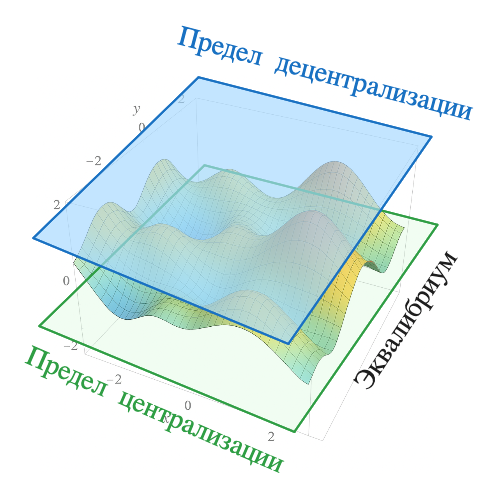
\includegraphics[width=0.5\textwidth]{./assets/de-centralization.png}
  \caption{Сравнение предел централизации и придела децентрализации}
  \label{fig:de-centralization}
\end{figure}

% ## 3.4
\mysection{Вывод по третей главе}

Таким образом, разработан механизм, сочетающий стимулы, рациональность агентов и доверенный механизм согласования, что позволяет эффективно распределять ресурсы на основе коллективных прогнозов.

С практической стороны ангелы-инвесторы предоставляют ликвидность авторам стартапов. В зависимости от результата проекта авторы могут выкупать токены полностью, частично или не выкупать совсем. Инвесторы защищены механизмом частичного возврата инвестиций при провале проекта.

% ###################################################
% ## Глава 4
\mychapter{РАЗРАБОТКА ДЕЦЕНТРАЛИЗОВАННОГО ПРИЛОЖЕНИЯ}
% ###################################################

% ## 4.1
\mysection{Описание бизнес-процессов}

% ### 4.1.1
\mysubsection{Функциональные требования к приложению}

\begin{itemize}
  \item \textbf{Функциональные требования:}
        \begin{itemize}
          \item Возможность записи и публикации видеопитчей
          \item Административная валидация питчей через Telegram
          \item Возможность просмотра, оценки и инвестирования в видеопитчи инвесторами
          \item Управление инвестиционным портфелем с отображением статистики
        \end{itemize}

  \item \textbf{Нефункциональные требования:}
        \begin{itemize}
          \item Производительность: отклик приложения не должен превышать 3 секунд
          \item Масштабируемость: приложение должно обеспечивать работу не менее 1000 одновременных пользователей
          \item Безопасность: смарт-контракты не должны содержать уязвимостей для управления ресурсами пользователей системы
          \item Юзабилити: простой и понятный интерфейс с интуитивной навигацией
          \item Совместимость: поддержка платформ iOS, Android, Telegram Mini Apps, Web
        \end{itemize}
\end{itemize}

% ### 4.1.2
\mysubsection{Разработать пользовательские сценарии}

% ### 4.1.3
\mysubsection{UML-модель механизма распределения ресурсов}

Для более наглядного представления модели распределения ресурсов в приложении была разработана UML-диаграмма вариантов использования (use case diagram), представленная на рисунке \ref{fig:uml-use-case-diagram}. Данная диаграмма демонстрирует взаимодействие различных акторов системы и распределение ролей между алгоритмическими и человеческими компонентами.

\begin{figure}[ht]
  \centering
  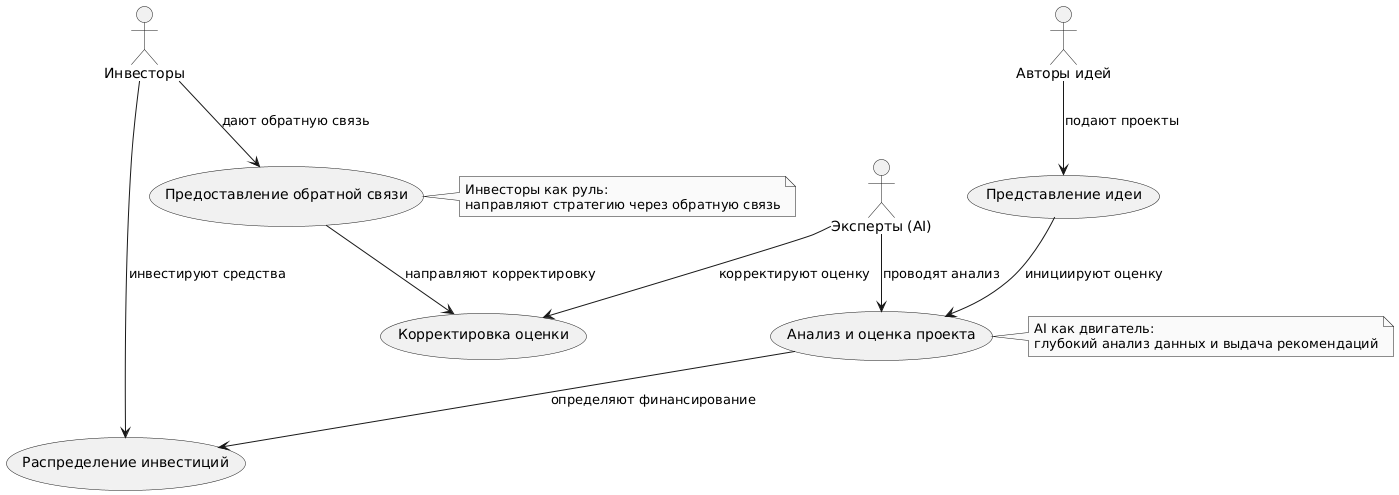
\includegraphics[width=0.9\textwidth]{./assets/uml-use-case-diagram.png}
  \caption{UML-диаграмма вариантов использования механизма распределения ресурсов с балансом автоматизации и человеческого контроля}
  \label{fig:uml-use-case-diagram}
\end{figure}

Как видно из диаграммы, в системе выделяются три основных группы участников: инвесторы, авторы идей и эксперты (представленные, в том числе, системами ИИ). Инвесторы участвуют в процессе предоставления обратной связи и непосредственного инвестирования средств, что направляет стратегию распределения ресурсов. Авторы идей подают свои проекты на рассмотрение через механизм представления идеи. Эксперты, включая аналитические системы на основе ИИ, выполняют ключевую роль по анализу и оценке проектов, а также корректировке предварительных оценок.

Центральными процессами в системе являются:

\begin{enumerate}
  \item Представление идеи -- процесс, при котором авторы формулируют и загружают свои проекты в систему с защитой интеллектуальной собственности.

  \item Анализ и оценка проекта -- основная аналитическая работа по многомерной оценке потенциала проекта, выполняемая в значительной степени автоматизированными системами с глубоким анализом данных.

  \item Предоставление обратной связи -- процесс, в котором инвесторы выражают свои предпочтения и видение направления развития.

  \item Корректировка оценки -- механизм коррекции и уточнения, где эксперты и инвесторы могут скорректировать предварительные результаты анализа.

  \item Распределение инвестиций -- финальный этап, на котором средства распределяются между проектами на основе комплексной оценки, полученной в результате работы механизма.
\end{enumerate}

Особенно важно отметить, что механизм построен по принципу, где алгоритмические компоненты выполняют основную вычислительную работу по обработке больших объемов данных, а человеческие компоненты направляют стратегию через обратную связь, определяют стратегические приоритеты и осуществляют контроль. Такой подход обеспечивает баланс эффективности и надежности, сочетая вычислительную мощь алгоритмов с ценностями и экспертизой человеческих участников.

Данный механизм реализует принцип коллективного принятия решений, где автоматизация используется для обеспечения объективности и масштабируемости, а человеческое участие – для стратегического управления процессом и сохранения этических аспектов распределения ресурсов.

\mysubsection{Процессная модель масштабированного механизма инвестирования}

В целях формализации и визуализации бизнес-процессов функционирования масштабированного механизма инвестирования была разработана BPMN-диаграмма (Business Process Model and Notation), представленная на рисунке \ref{fig:bpmn}. Данная диаграмма иллюстрирует композицию взаимодействий между ключевыми участниками системы и последовательность выполняемых операций в рамках полного инвестиционного цикла.

\begin{figure}[h]
  \centering
  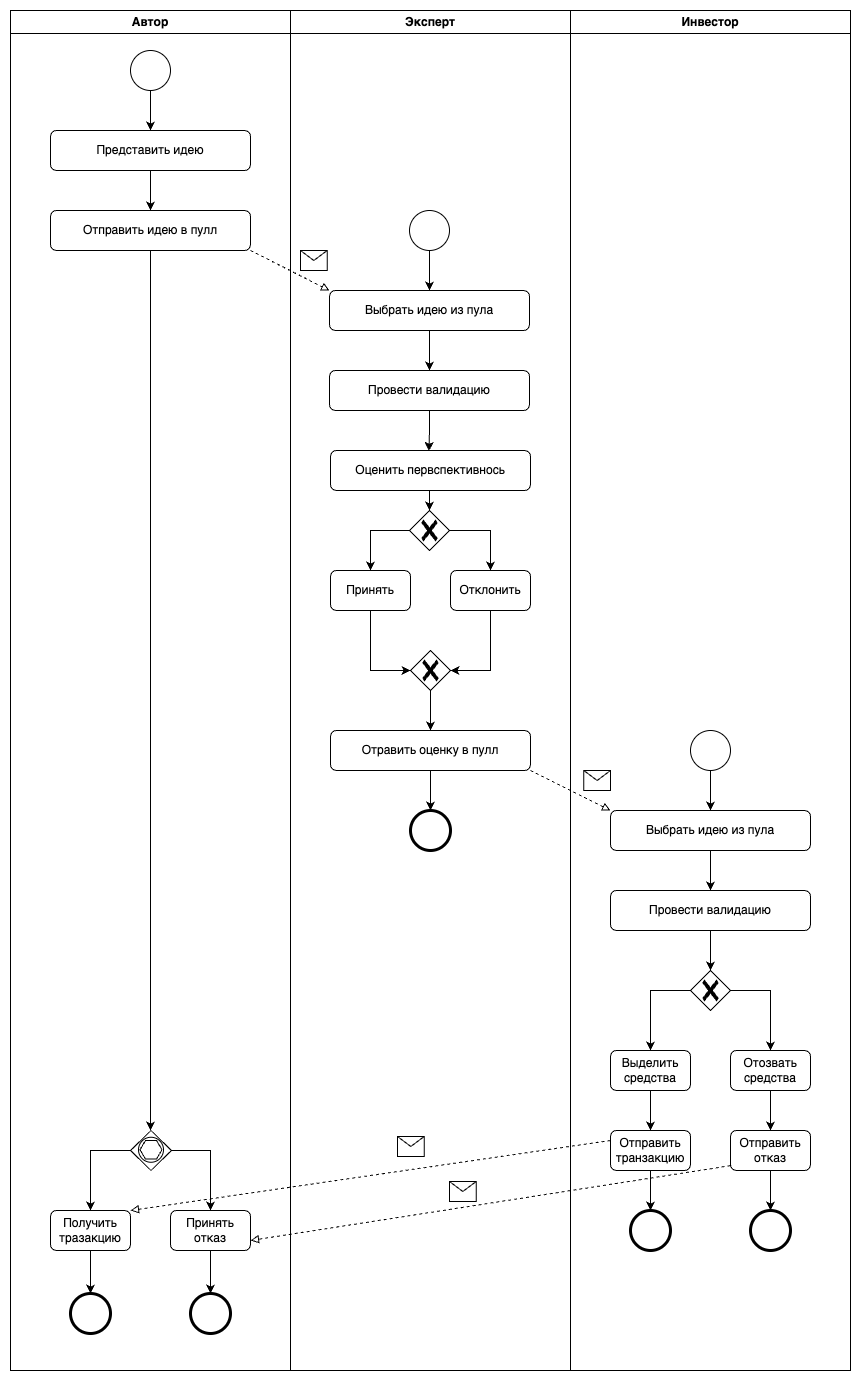
\includegraphics[width=0.5\textwidth]{./assets/bpmn.drawio.png}
  \caption{BPMN-диаграмма процессов масштабированного механизма инвестирования}
  \label{fig:bpmn}
\end{figure}

Информационное взаимодействие между пулом авторов и пулом экспертов осуществляется посредством асинхронных сообщений, что отражает передачу метаданных проекта без раскрытия его полного содержания. В пуле экспертов активируется комплексный подпроцесс, включающий выбор идеи из общего пула, проведение валидации представленных данных и многомерную оценку перспективности проекта. Этот этап реализуется с применением аналитического движка на основе искусственного интеллекта, который обрабатывает структурированные данные проекта с использованием ансамблевых методов машинного обучения. Диаграмма отражает ключевой шлюз (gateway) принятия решения, где эксперт формирует заключение о перспективности идеи на основе результатов аналитического движка и собственной экспертизы. Данное решение может иметь положительный или отрицательный характер, однако в обоих случаях процесс конвергирует к операции отправки оценки в общий пул, что завершает участие эксперта в текущем инвестиционном цикле.

Далее информационный поток направляется к пулу инвесторов, где инициируется подпроцесс выбора и независимой валидации идеи. Центральным элементом данного этапа является шлюз принятия инвестиционного решения, за которым следуют дивергентные пути процесса: выделение средств или отказ от инвестирования. В случае положительного решения активируется последовательность операций финансирования с использованием механизмов квадратичного финансирования и возрастающих кривых ограничения, реализованных посредством смарт-контрактов в выбранной блокчейн-инфраструктуре. При отрицательном решении формируется и отправляется уведомление об отказе.

Заключительный этап процесса визуализируется возвращением информационного потока к пулу автора, где происходит финальное разветвление процесса в зависимости от полученного результата: получение транзакции либо обработка отказа. Оба пути завершаются соответствующими конечными событиями, отражающими завершение инвестиционного цикла для конкретного проекта.

Особого внимания заслуживают интегрированные в диаграмму элементы, отражающие механизмы масштабирования платформы. На уровне технологической инфраструктуры визуализируется применение решений второго уровня (Layer 2) для блокчейна Ethereum, что обеспечивает высокую пропускную способность системы при сохранении базового уровня безопасности. Данный подход позволяет поддерживать растущий объем транзакций без существенного увеличения операционных издержек, что критически важно для развития платформы. Параллельно отображаются процессы мониторинга производительности и автоматического масштабирования вычислительных ресурсов, обеспечивающие адаптивность системы к флуктуирующим нагрузкам.

Диаграмма также отражает ключевые подпроцессы, связанные с обеспечением безопасности и целостности данных, включая распределенное хранение зашифрованной информации в IPFS, применение мультисигнатурных механизмов для критических операций и регулярное резервное копирование состояния системы. Интеграция с внешними сервисами и API визуализируется посредством элементов сервисных задач, подчеркивая взаимодействие системы с внешними компонентами экосистемы.

В контексте управления процессом масштабирования значительную роль играют механизмы обратной связи, позволяющие оперативно корректировать параметры функционирования системы на основе получаемых метрик эффективности. Эти механизмы представлены на диаграмме в виде циклических потоков, соединяющих аналитические процессы с процессами принятия решений о параметрической оптимизации системы.

Таким образом, разработанная BPMN-диаграмма представляет собой комплексное формализованное описание функционирования масштабированного механизма инвестирования, интегрирующее как бизнес-логику взаимодействия ключевых участников, так и технологические аспекты, обеспечивающие масштабируемость, безопасность и адаптивность платформы в условиях возрастающей нагрузки и расширяющегося функционала.

\mysection{Архитектура платформы и основные компоненты}

Архитектура платформы инвестирования разработана с учётом принципов децентрализации, безопасности, масштабируемости, что позволило интегрировать технологии блокчейна, искусственного интеллекта и современные криптографические механизмы в единую систему, способную обеспечить эффективное и справедливое распределение капитала для финансирования инновационных проектов. Данная архитектура построена на модульном принципе, когда различные компоненты, оставаясь взаимосвязанными, функционируют независимо, что обеспечивает гибкость системы и возможность эволюционного развития отдельных её частей. В основе проектирования лежит идея распределения критически важных данных и сервисов по сети, что устраняет единую точку отказа и позволяет обеспечить устойчивость к цензуре, а также применение криптографических методов и принципа минимального необходимого доступа, что гарантирует безопасность и защиту конфиденциальной информации. Кроме того, система сконструирована таким образом, чтобы сохранять высокую производительность при увеличении количества обрабатываемых проектов и пользователей, что достигается за счёт применения решений второго уровня для блокчейна и распределённых вычислений для реализации алгоритмов искусственного интеллекта. Применение открытых стандартов и протоколов способствует созданию интероперабельной среды, а механизмы коллективного управления обеспечивают адаптивность архитектуры к изменяющимся требованиям.

Базовый уровень архитектуры включает слой блокчейна, отвечающий за запись и верификацию транзакций, исполнение смарт-контрактов и токенизацию активов, а также протокольный слой, в котором реализуются специализированные алгоритмы защиты интеллектуальной собственности, квадратичного финансирования и возрастающих кривых ограничения. Дополнительные слои отвечают за аналитику и обработку данных с использованием искусственного интеллекта, а также за предоставление удобного пользовательского интерфейса, что позволяет участникам системы взаимодействовать с платформой на различных уровнях доступа. При этом интеграция с внешними системами, базами данных и другими блокчейн-платформами расширяет функциональные возможности всей системы.

Ключевые компоненты системы охватывают комплексное управление проектами, инвестиционный механизм, аналитический движок, систему защиты интеллектуальной собственности, платформу децентрализованного управления, а также интерфейсы и API для взаимодействия с внешними сервисами. Функциональность управления проектами реализуется посредством представления и категоризации идей, сопровождаемой механизмами проверки качества и верификации данных, что обеспечивает конфиденциальное взаимодействие между основателями и инвесторами. Инвестиционный механизм базируется на математически обоснованных схемах токенизации и распределения ресурсов, позволяющих оптимизировать финансирование посредством квадратичного механизма и защиты от атак, включая атаки Сибиллы, посредством специально разработанных смарт-контрактов. Аналитический движок, построенный на современных моделях искусственного интеллекта, позволяет проводить комплексный анализ потенциала проектов, оценивать рыночные тренды, выявлять закономерности и прогнозировать успешность проектов. В свою очередь, система защиты интеллектуальной собственности включает в себя современные криптографические протоколы, такие как доказательства с нулевым разглашением, а также механизмы временного закрепления информации на блокчейне и безопасной многосторонней вычислимости. Организация децентрализованного управления посредством DAO, поддерживаемая механизмами голосования и системы репутации, позволяет обеспечить прозрачное и гибкое управление платформой, а разработанные интерфейсы и API делают систему доступной для широкого круга пользователей.

При выборе стека технологий основное внимание уделялось использованию EVM-совместимых блокчейнов для реализации смарт-контрактов, а также решений второго уровня, способствующих повышению масштабируемости и снижению транзакционных издержек. В качестве языков программирования для смарт-контрактов применялись Solidity и Vyper, а разработка сопровождалась использованием проверенных фреймворков, таких как Hardhat и OpenZeppelin. Современные криптографические методы, включая zk-SNARKs и zk-STARKs, обеспечивают защиту конфиденциальной информации, а применение IPFS с шифрованием гарантирует безопасность хранения данных. Реализация алгоритмов искусственного интеллекта осуществлялась на базе фреймворков TensorFlow и PyTorch с применением моделей обработки естественного языка и графовых нейронных сетей, что обеспечивает высокую точность анализа. В серверной части использовались технологии Node.js, Python, GraphQL, Redis и PostgreSQL, а фронтенд разработка осуществлялась с применением React.js и ethers.js, что позволило создать современный и удобный пользовательский интерфейс. Важное значение имели инструменты контейнеризации и оркестрации, такие как Docker и Kubernetes, а также облачные решения, позволяющие обеспечить отказоустойчивость и масштабируемость всей системы.

\mysection{Разработка ядра системы}

Код смарт-контакта представлен в листинге \ref{lst:rlmodel}.

\begin{lstlisting}[language=Python, caption={Пример кода}, label={lst:rlmodel}]
  def example_function():
      return "Hello from Listing"
  \end{lstlisting}

\mysubsection{Механизм оценки проектов с использованием искусственного интеллекта}

Механизм оценки проектов представляет собой ключевой компонент платформы, направленный на проведение объективного анализа потенциала инновационных идей без раскрытия конфиденциальных данных. Данный механизм объединяет алгоритмы искусственного интеллекта с принципами дистиллированного человеческого суждения, что позволяет создать систему, сочетающую масштабируемость автоматизированного анализа и экспертное понимание. В основе данного подхода лежит структурированное представление проектов, в рамках которого публичные метаданные характеризуют отрасль, категорию, целевой рынок, стадию развития, ключевые показатели и модель монетизации, а также временные вехи развития, что даёт возможность инвесторам проводить оценку на основе агрегированных данных. Наряду с этим, защищённые данные, включающие детальное техническое описание, уникальные технологические решения и аспекты реализации, обрабатываются отдельно с применением современных методов защиты интеллектуальной собственности. Важным элементом является также формирование доказательств конкурентных преимуществ посредством криптографических методов нулевого разглашения, что позволяет подтвердить уникальность решения и его инновационный потенциал без раскрытия конфиденциальной информации. Для алгоритмической обработки проектов используются векторные представления идей и структурированные данные, что обеспечивает объективность сравнительного анализа и повышает точность итоговой оценки.

Разработанная многомерная модель оценки охватывает анализ инновационности, рыночного потенциала, технической выполнимости, бизнес-модели и конкурентной среды. Оценка инновационности осуществляется через сравнительный анализ новизны идеи, её потенциального влияния на отрасль и выявление уникальных методологических подходов \cite{stanley2015greatness}. Анализ рыночного потенциала базируется на оценке динамики целевого рынка, соответствия современным трендам и прогнозировании спроса, тогда как оценка технической выполнимости опирается на реалистичность предложенных технических решений и выявление возможных барьеров в реализации. Кроме того, анализ бизнес-модели позволяет оценить эффективность, устойчивость и потенциал масштабирования, а изучение конкурентной среды помогает определить наличие существенных конкурентных преимуществ и барьеров входа на рынок. Для каждого из этих направлений используются специализированные алгоритмы, в том числе нейронные сети глубокого обучения, графовые и рекуррентные нейронные сети, а также ансамблевые методы, что в совокупности позволяет агрегировать результаты анализа в единую оценку, применимую для принятия инвестиционных решений.

Особое внимание уделяется обучению моделей на исторических данных, что включает сбор информации о стартапах на различных стадиях, данные о финансировании, отраслевые тренды и текстовые описания проектов. Процесс предобработки данных включает стандартизацию, нормализацию, обработку пропущенных значений, балансировку классов и аугментацию информации для обеспечения репрезентативности обучающих выборок. В ходе обучения используются методы кросс-валидации, оптимизация гиперпараметров и ансамблирование, что позволяет снизить риск систематических ошибок и предвзятости, а постоянное обновление моделей посредством механизмов обратной связи гарантирует адаптацию системы к изменяющимся рыночным условиям. Интеграция дистиллированного человеческого суждения реализована посредством калибровки моделей с участием опытных экспертов, совместного принятия решений и обучения с подкреплением на основе обратной связи, что позволяет комбинировать алгоритмическую эффективность с экспертной интуицией и повышать объективность оценок.

См. рисунок \ref{fig:database} для дополнительной информации.

\begin{figure}[h]
  \centering
  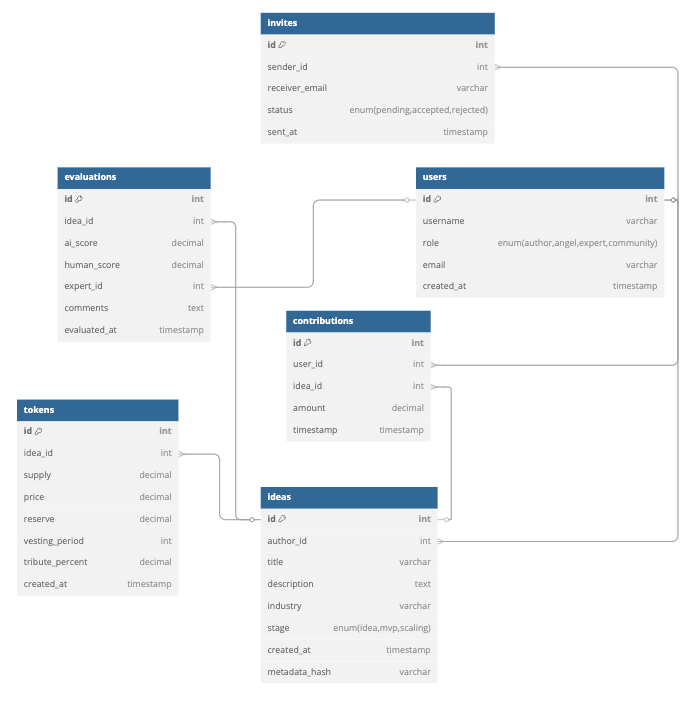
\includegraphics[width=0.5\textwidth]{./assets/database.png}
  \caption{{\protect\hyperlink{fig:database}{Схема базы данных}}}
  \label{fig:database}
\end{figure}

База данных разработанна как локальная оффчейн-система для мобильного приложения и предназначена для поддержки работы платформы, которая решает задачи инвестирования в ранние стадии стартапов через слепые инвестиции и технологии блокчейна. Центральной таблицей является таблица пользователей, которая содержит информацию о всех участниках платформы — авторах идей (предпринимателях), инвесторах, экспертах и членах сообщества. В этой таблице хранятся уникальные идентификаторы пользователей, их имена, роли (автор, инвестор, эксперт или участник сообщества), электронные адреса и даты регистрации, что позволяет отслеживать взаимодействие каждого участника с платформой.

Таблица идей служит для безопасного хранения зашифрованных идей стартапов на устройствах пользователей до момента их токенизации на блокчейне. Она включает уникальные идентификаторы идей, ссылки на авторов из таблицы пользователей, названия и подробные описания идей (зашифрованные для защиты интеллектуальной собственности), а также информацию об отрасли, стадии развития (идея, MVP или масштабирование), дате создания и хеше метаданных, который используется для последующей верификации на блокчейне. Эта таблица связана с таблицей пользователей через авторов идей, а также с другими таблицами для оценки, финансирования и токенизации.

Таблица оценок фиксирует результаты анализа идей, проводимого искусственным интеллектом и людьми, что обеспечивает слепую и объективную оценку для инвестиционных решений. В ней хранятся уникальные идентификаторы оценок, ссылки на оцениваемые идеи, баллы, вычисленные ИИ, и корректировки, внесенные экспертами или сообществом, а также комментарии и даты проведения оценок. Эта таблица связана с таблицей идей (через оцениваемые идеи) и таблицей пользователей (через экспертов, проводящих оценку).

Таблица вкладов регистрирует локальные финансовые вложения пользователей в идеи до их токенизации на блокчейне. Она включает уникальные идентификаторы вкладов, ссылки на пользователей, вносящих средства, и идеи, получающие финансирование, суммы вкладов в местной валюте или криптовалюте, а также даты и время внесения. Эта таблица связывает пользователей и идеи, обеспечивая отслеживание финансовой поддержки.

Таблица токенов управляет локальными данными о токенах, которые будут токенизированы на блокчейне после инвестиций. В ней хранятся уникальные идентификаторы токенов, ссылки на связанные идеи, начальный объем эмиссии, текущую цену (рассчитанную по механизму возрастающих кривых ограничения), резервный пул для финансирования идей, период вестинга (например, 180 дней) и процент трибута (например, 10\%) для резерва. Таблица связана с таблицей идей, поддерживая механизм распределения ресурсов.

Наконец, таблица приглашений поддерживает систему эксклюзивности и сообщества, фиксируя приглашения, отправленные между пользователями. Она содержит уникальные идентификаторы приглашений, ссылки на отправителей из таблицы пользователей, электронные адреса получателей, статус приглашения (ожидает, принято, отклонено) и дату отправки. Эта таблица связана с таблицей пользователей, обеспечивая управление сетью участников.

Все таблицы базы данных тесно взаимосвязаны: пользователи связаны с идеями через авторов, с оценками через экспертов, с вкладами через инвесторов и с приглашениями через отправителей и получателей. Идеи, в свою очередь, связаны с оценками, вкладами, токенами и пользователями, создавая единую экосистему для слепых инвестиций, объективной оценки и защиты интеллектуальной собственности на локальном уровне до передачи данных на блокчейн. Такая структура поддерживает ключевые функции платформы, включая конфиденциальность, объективность и масштабируемость для широкого круга пользователей — авторов и инвесторов.


% ## 4.4
\mysection{Разработка серверной части}


% ## 4.5
\mysection{Разработка клиентской части}

Интерфейс прототипа разработан с учетом принципов интуитивности и простоты взаимодействия, обеспечивая при этом доступ ко всему функционалу системы.
Общая схема взаимодействия компонентов прототипа представлена на рисунке \ref{fig:app-prototype}, где проиллюстрированы основные процессы и связи между элементами системы.

\begin{figure}[h]
  \centering
  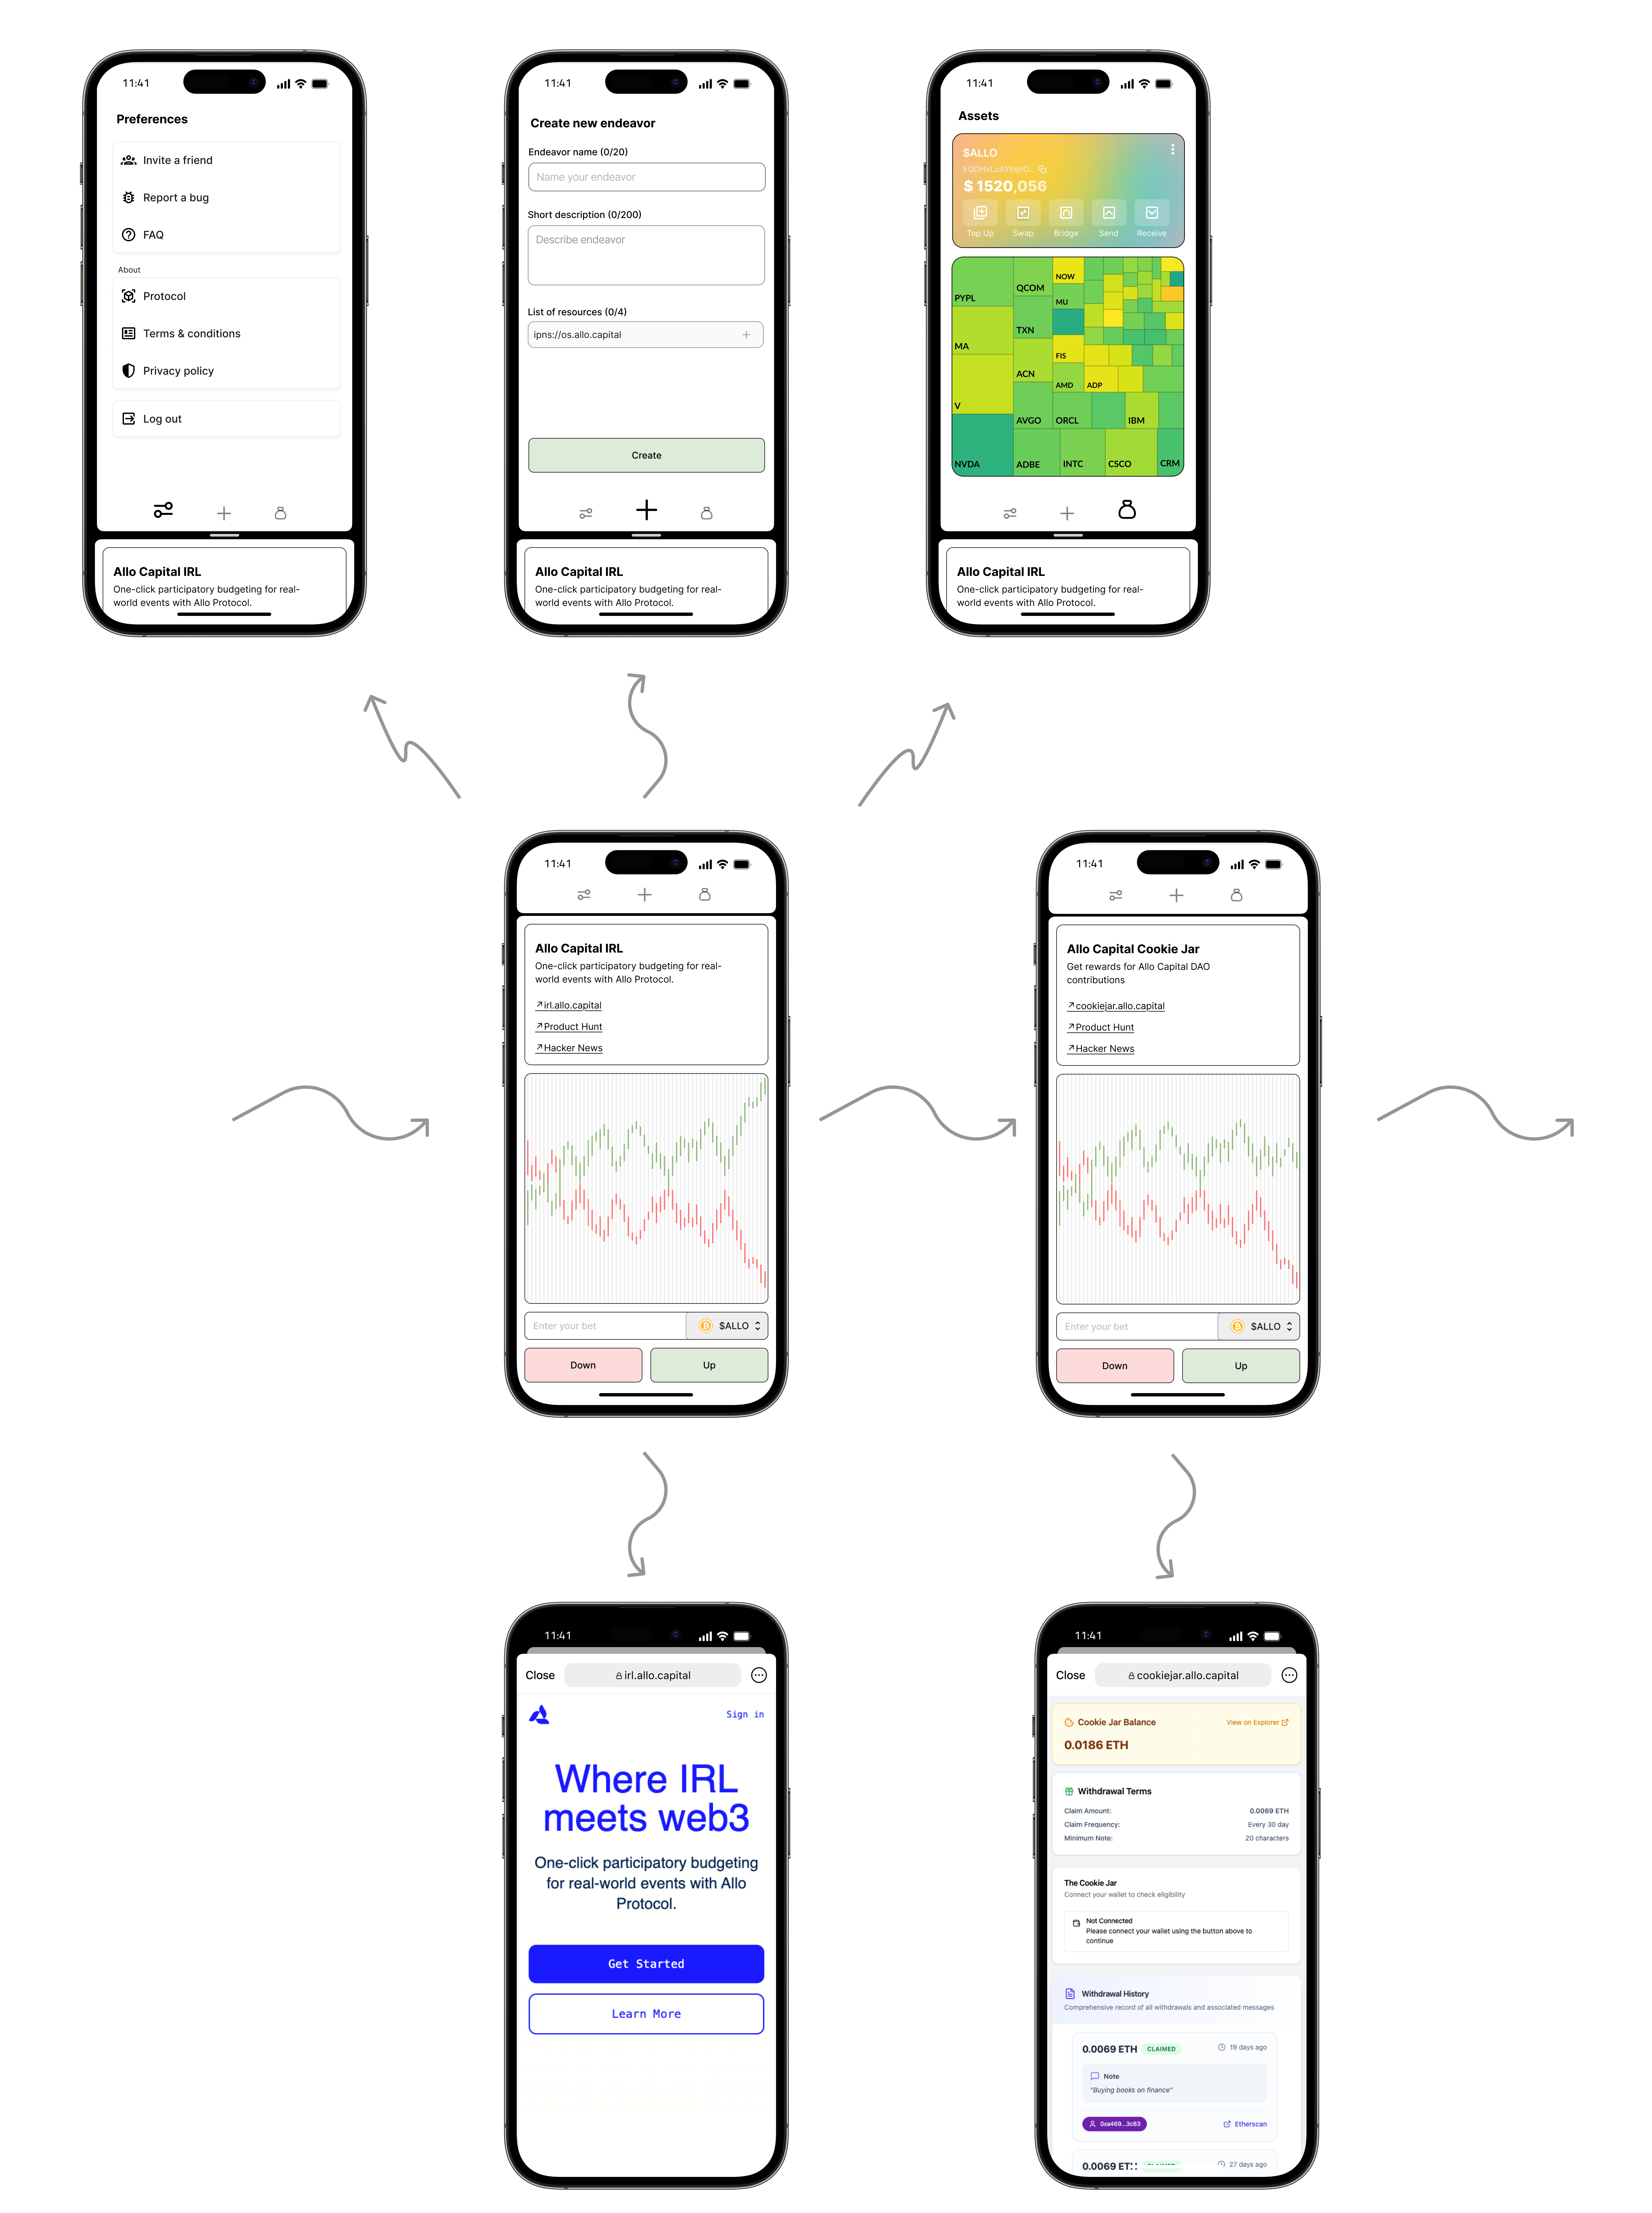
\includegraphics[width=0.5\textwidth]{./assets/app-prototype.png}
  \caption{Схема основных процессов и взаимодействий в прототипе платформы}
  \label{fig:app-prototype}
\end{figure}

% ### 4.5.1
\mysubsection{Главный экран приложения}

Основной сценарий использования приложения. На нём отображается ключевая информация и основные действия, доступные сразу после запуска. В верхней части располагается заголовок приложения или логотип, а также кнопки навигации (например, кнопка меню для перехода к экрану навигации между модулями).

Центральное пространство главного экрана отведено под список текущих инициатив или проектов. Каждая инициатива представлена в виде карточки или строки: содержит название инициативы и её краткое описание. В прототипе на карточке отображается название проекта и одна строка с описанием его цели или сути. Кроме того, под описанием располагаются иконки или ссылки на внешние ресурсы, связанные с этой инициативой (например, иконки Product Hunt или Hacker News, если инициатива упоминается на этих платформах).

% Face disclosure +3%
% https://www.mdpi.com/2227-9091/12/10/165?utm_source=chatgpt.com

Основное назначение главного экрана – предоставить пользователю обзор актуальных инициатив и быстрый доступ к дальнейшим действиям. Пользователь может прокручивать список для просмотра всех доступных инициатив. Нажатие на карточку инициативы приводит к переходу на экран браузера, где раскрываются подробности выбранного проекта в виде встроенной веб-страницы.

С главного экрана также доступен переход к созданию новой инициативы – это реализовано через отдельную кнопку (значок "+" на панели) или через меню навигации. Пример отображения главного экрана приведён на рисунке \ref{fig:app-main-flow}.

\begin{figure}[h]
  \centering
  
\includegraphics[width=0.5\textwidth]{./assets/app-main-flow.png}
  \caption{Главный экран приложения со списком инициатив}
  \label{fig:app-main-flow}
\end{figure}

\mysubsection{Экран браузера}

Экран браузера предназначен для отображения детальной информации об инициативе посредством встроенного веб-браузера. Этот экран открывается, когда пользователь выбирает инициативу на главном экране или нажимает на связанный с ней внешний ресурс.

В верхней части экрана браузера присутствует панель навигации: она содержит кнопку «Назад» для возвращения к предыдущему экрану (например, обратно к главному списку) и отображает адрес или название ресурса, который просматривается. Основное пространство занимает содержимое веб-страницы, связанной с выбранной инициативой.

В прототипе при открытии инициативы пользователь видит встроенную страницу с подробным описанием проекта: заголовок, расширенное описание, мультимедийные материалы и кнопки взаимодействия (такие как «Get Started», «Learn More»).

Во время просмотра встроенной страницы пользователь может взаимодействовать с ней так же, как в обычном браузере: прокручивать контент, нажимать на ссылки или кнопки. При этом, благодаря встроенному браузеру, нет необходимости покидать приложение. Пример экрана браузера представлен на рисунке \ref{fig:app-browser}.

\begin{figure}[h]
  \centering
  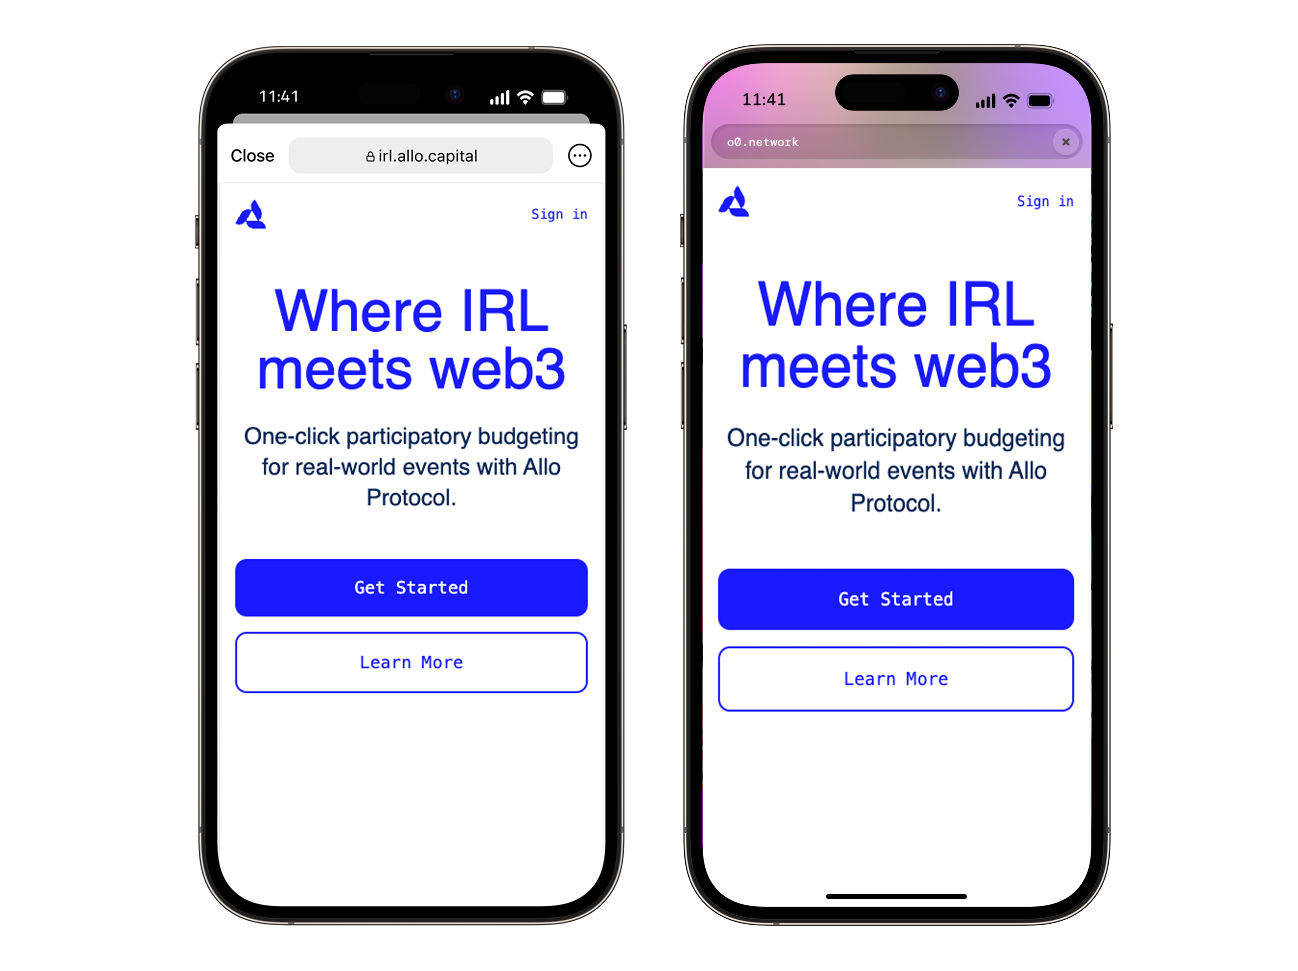
\includegraphics[width=0.5\textwidth]{./assets/app-browser.png}
  \caption{Пример экрана браузера с детальной информацией о проекте}
  \label{fig:app-browser}
\end{figure}

В появившемся меню отображается список пунктов, позволяющих перейти к различным экранам: например, к экрану управления активами, к экрану создания новой инициативы, к профилю или настройкам. В верхней части навигационного меню показывается профиль пользователя (имя, аватар) или название приложения, а ниже перечислены основные разделы.

В прототипе меню навигации содержит пункты: «Assets» (Активы) для перехода к финансовым показателям, «Create new endeavor» (Создать инициативу) для запуска экрана создания проекта, а также ряд пунктов, связанных с настройками пользователя и информацией о системе. Например, в меню присутствуют элементы «Preferences» (Настройки), «Invite a friend» (Пригласить друга), «Report a bug» (Сообщить об ошибке), «FAQ» (Частые вопросы), «About» (О приложении), «Protocol» (Информация о протоколе платформы), «Terms \& conditions» (Пользовательское соглашение), «Privacy policy» (Политика конфиденциальности) и «Log out» (Выход из аккаунта).

Пример экрана навигации показан на рисунке \ref{fig:app-navigation}, где представлены различные модули доступные пользователю.

\begin{figure}[h]
  \centering
  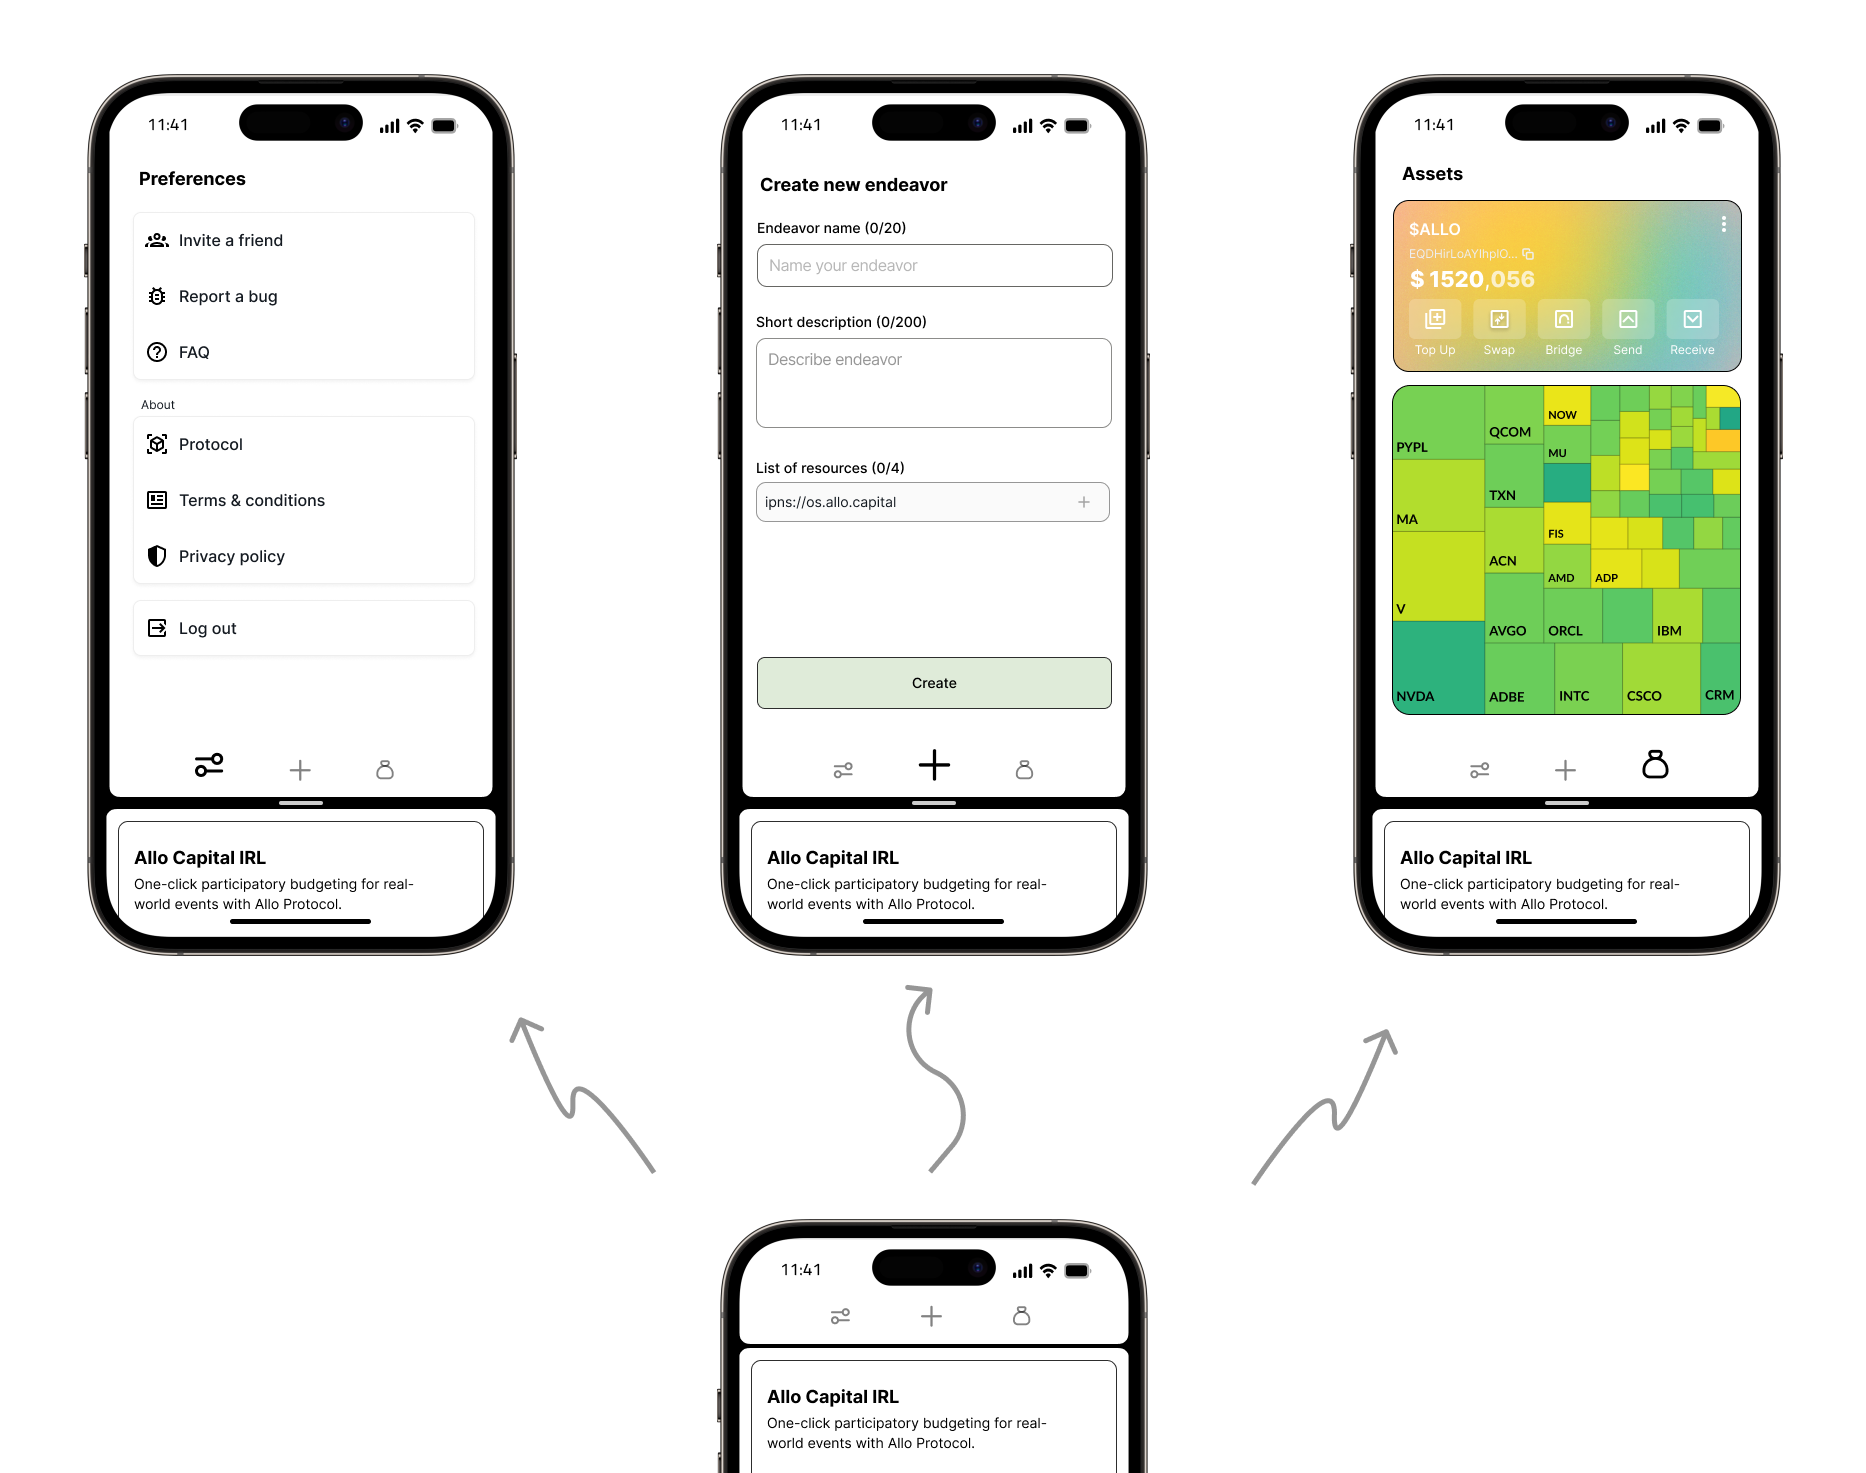
\includegraphics[width=0.5\textwidth]{./assets/app-navigation.png}
  \caption{Экран навигации между модулями приложения}
  \label{fig:app-navigation}
\end{figure}

% #### 4.5.2
\mysubsection{Экран управления активами и финансами}

Экран управления активами предоставляет пользователю сведения о его финансовых ресурсах в приложении. Здесь отображаются все доступные активы (например, внутренние токены или валюты, связанные с платформой).

Интерфейс организован в виде списка кошельков или счетов: каждая строка представляет отдельный актив с указанием его названия или тикера, идентификатора (например, часть адреса кошелька) и текущего баланса. В прототипе присутствует актив с кодом \$ALLO — рядом с ним показан уникальный идентификатор (адрес счёта или номер кошелька) и баланс, выраженный числом (например, 1,520,056).

Для каждого актива предусмотрены отдельные управляющие элементы: кнопки действий для управления средствами, такие как «Top Up» (пополнить), «Swap» (обменять), «Bridge» (перевести между сетями), «Send» (отправить) и «Receive» (получить). Ниже основного актива также отображается тепловая карта инвестиций по различным проектам, что позволяет пользователю визуально оценить распределение своих активов.

Типичный сценарий использования: пользователь переходит в этот раздел, чтобы проверить достаточен ли у него баланс для участия в той или иной инициативе, либо чтобы просмотреть результаты предыдущих взаимодействий.

% #### 4.5.3
\mysubsection{Экран создания новой инициативы}

Экран создания новой инициативы позволяет пользователю добавить свой собственный проект или предложение в систему. Это форма ввода данных, где последовательно представлены поля, необходимые для описания инициативы.

На экране отображается заголовок формы «Create new endeavor» (Создать новую инициативу) для ясности. Далее следуют поля ввода: первое поле – название инициативы, ограниченное определённым количеством символов (в прототипе указано ограничение 0/20 символов, что означает максимальную длину имени 20 символов). Следующее поле – краткое описание инициативы (с ограничением 0/200 символов).

Затем присутствует блок для добавления связанных ресурсов или ссылок. В прототипе есть раздел «List of resources (0/4)», куда пользователь может добавить до четырёх ссылок на внешние ресурсы, связанные с инициативой. Один из примеров такого ресурса показан как ссылка на распределенное хранилище или страницу проекта.

После заполнения необходимых полей активируется кнопка «Create» (Создать), расположенная в нижней части формы. Нажатие этой кнопки сохраняет новую инициативу. Приложение при этом выполняет валидацию введённых данных и создает запись инициативы в системе.

% #### 4.5.4
\mysubsection{Экран настроек пользователя}

Экран настроек пользователя содержит опции для персонализации и обслуживания аккаунта. Этот раздел включает различные пункты, сгруппированные по тематике. В прототипе часть этих пунктов уже видна в меню навигации: например, «Preferences» (общие настройки), «Invite a friend» (приглашение новых пользователей), «Report a bug» (сообщение об ошибке разработчикам), «FAQ» (ответы на частые вопросы), и другие.

На экране настроек эти пункты представлены списком кнопок или ссылок. Нажатие на каждый из них приводит к соответствующему действию или открывает дополнительную информацию. Например, выбор «Preferences» открывает подэкран с настройками (переключателями и опциями, такими как уведомления, язык интерфейса). Выбор «Invite a friend» вызывает окно шаринга или копирует реферальную ссылку.

Экран настроек также отвечает за связь пользователя с системой в целом. Здесь расположен пункт «Log out» (Выход), с помощью которого пользователь может выйти из своего аккаунта или отключить текущую сессию.

С точки зрения сценариев, пользователь обращается к экрану настроек по необходимости: изменить что-то в профиле, узнать информацию о приложении, связаться с поддержкой или выйти из системы. Пример экрана настроек можно увидеть на рисунке.

Все представленные экраны в совокупности формируют комплексное пользовательское взаимодействие с платформой, обеспечивая доступ ко всему функционалу системы через интуитивно понятный мобильный интерфейс.

% ## 4.7
\mysection{Вывод по четвертой главе}


% ###################################################
% ## Глава 5
% ###################################################

\mychapter{ПЕРСПЕКТИВЫ РАЗВИТИЯ}

\mysection{Масштабирование инвестиционной платформы}


Монетизация системы может происходить за счёт стейкинга пула ликвидности, а управление механизмом в перспективе может быть реализовано посредством community notes. В долгосрочной перспективе возможен выпуск стейблкоинов, обеспеченных пулами ликвидности и привязанных к стабильным активам, что значительно расширит функционал и доступность системы для пользователей и инвесторов.

Дальнейшее развитие платформы инвестирования организовано в виде последовательного поэтапного процесса, каждый этап которого имеет чётко определённые цели, задачи и показатели успеха. На первой фазе создаётся минимально жизнеспособный продукт, направленный на проверку ключевых концепций, привлечение ограниченной группы ранних пользователей, сбор первичной обратной связи и валидацию основных гипотез. В этот период реализуются базовые механизмы квадратичного финансирования, протоколы защиты интеллектуальной собственности и первичные пользовательские интерфейсы, что позволяет провести серию тестовых раундов финансирования и определить направления дальнейшего развития. Вторая фаза предусматривает запуск полнофункциональной версии платформы в основной сети, расширение аудитории посредством целевого маркетинга, оптимизацию операционных процессов и формирование сообщества, при этом реализуются более продвинутые версии ключевых механизмов, что позволяет обеспечить выполнение запланированных финансовых и эксплуатационных показателей. Третья фаза направлена на масштабирование функциональности и интеграцию с существующими экосистемами венчурного финансирования, что включает международную экспансию, адаптацию экономических механизмов на основе эмпирических данных и глубокую интеграцию с традиционными инвестиционными платформами, что приводит к значительному росту числа активных пользователей и объёмов привлечённого капитала. Четвёртая фаза предусматривает переход к полностью децентрализованной модели управления, создание открытой экосистемы для сторонних разработчиков, достижение самодостаточности экономической модели и становление платформы в качестве отраслевого стандарта для инвестирования в ранних стадиях инновационных проектов.

Стратегия масштабирования технологической инфраструктуры базируется на поэтапном увеличении вычислительных мощностей, расширении блокчейн-инфраструктуры, оптимизации систем хранения данных и сетевых решений. При этом особое внимание уделяется постепенному увеличению резервных мощностей, модульности отдельных компонентов и автоматическому выделению ресурсов в зависимости от текущих потребностей системы. В начальной фазе используется развертывание на Ethereum Layer 2 для баланса между безопасностью и транзакционными издержками, с последующим внедрением мультичейн-архитектуры и специализированных решений для оптимизации хранения данных и вычислений. Стратегия выхода на рынок строится на последовательном подходе, начиная с фокусирования на узких сегментах аудитории, таких как технологические стартапы и эксперты в области блокчейна, с последующим расширением до традиционных инвесторов и, наконец, до массового рынка. Привлечение пользователей осуществляется посредством специализированных демонстраций, программ раннего доступа, образовательных инициатив и масштабных маркетинговых кампаний, что позволяет постепенно формировать устойчивое и активное сообщество вокруг платформы. Эффективность данной стратегии оценивается с помощью ключевых метрик, таких как стоимость привлечения пользователя, коэффициент удержания, уровень вовлечённости и органический рост за счёт рекомендаций, что позволяет оперативно корректировать маркетинговые и технические решения.

\mysection{Обобщение результатов}


\mysection{Практическое применение}

Найм

Оценка проектов

Рассмотрим на примере контеста на Pond

Контест на pond является подобной средой со скрытым механизмом оценки

Можем выбрать архитектуру или метрики для LLM модель
Попробуем использовать LLM в качестве агента

\mysection{Вывод по пятой главе}

Соединение воедино открывает возможности для маштабирования
Разработка такой системы для блокчейн принесет приемущества и вероятно откроет не только экономические применения
(однако консенсус невозможен)


% ###################################################
% ## Заключение
% ###################################################

\newpage
\begin{center}
  \textbf{ЗАКЛЮЧЕНИЕ}
\end{center}
\addcontentsline{toc}{chapter}{ЗАКЛЮЧЕНИЕ}

В рамках данной дипломной работы была разработана и исследована платформа слепого инвестирования в ранние стадии стартапов, основанная на блокчейн-технологиях и искусственном интеллекте. Работа была направлена на решение структурных проблем существующей системы венчурного финансирования, включая информационную асимметрию, субъективность оценок и риски для интеллектуальной собственности.

Ключевые результаты, достигнутые в ходе работы:

1. Проведен комплексный анализ существующих механизмов инвестирования в ранние стадии, выявлены их преимущества и ограничения. Определены основные проблемы, препятствующие эффективному распределению капитала для инновационных проектов.

2. Изучены и адаптированы передовые концепции и механизмы, включая квадратичное финансирование, возрастающие кривые ограничения и механизм распределения ресурсов с балансом автоматизации и человеческого контроля. Разработаны модификации этих механизмов для специфического контекста инвестирования в ранние стадии.

3. Разработана архитектура платформы, обеспечивающая защиту интеллектуальной собственности, объективную оценку проектов и оптимальное распределение капитала. Архитектура включает модули для управления проектами, механизмы инвестирования, аналитические движки и системы защиты интеллектуальной собственности.

4. Обоснован выбор технологического стека, включающего блокчейн Ethereum с решениями Layer 2 для обеспечения масштабируемости, криптографические протоколы для защиты данных, фреймворки искусственного интеллекта для оценки проектов и современные технологии для разработки пользовательских интерфейсов.

5. Разработан прототип платформы с ключевыми механизмами, включая протоколы защиты интеллектуальной собственности, системы оценки проектов, механизмы квадратичного финансирования и возрастающие кривые ограничения.

6. Проведена комплексная оценка эффективности предложенной платформы, включающая технические, функциональные, пользовательские и экономические тесты. Предварительные результаты показывают потенциал для 28\% повышения эффективности распределения ресурсов по сравнению с традиционными механизмами.

7. Разработаны рекомендации по интеграции и масштабированию решения, включая дорожную карту развития, стратегию выхода на рынок и направления дальнейших исследований.

Практическая значимость разработанной платформы заключается в создании новой парадигмы инвестирования, которая имеет потенциал для преодоления структурных ограничений существующих механизмов и обеспечения более эффективного распределения ресурсов для инновационных проектов. Это может способствовать ускорению технологического развития, созданию новых рабочих мест и повышению глобальной конкурентоспособности экономики.

Проведенное исследование также выявило ряд направлений для дальнейшей работы, включая совершенствование криптоэкономических механизмов, развитие технологий защиты интеллектуальной собственности, улучшение методов оценки проектов, исследование социально-экономических эффектов и развитие регуляторных подходов.

В целом, результаты работы демонстрируют значительный потенциал интеграции блокчейн-технологий, искусственного интеллекта и инновационных экономических механизмов для трансформации системы венчурного инвестирования в направлении большей эффективности, справедливости и доступности. Разработанная платформа представляет собой не просто технологическое решение, но комплексный подход к переосмыслению процессов распределения ресурсов для инновационных проектов, что имеет стратегическое значение для развития экономики знаний и инноваций.

\renewcommand{\bibname}{\fontsize{14pt}{21pt}\selectfont СПИСОК ИСПОЛЬЗОВАННЫХ ИСТОЧНИКОВ}
\bibliographystyle{bibformat}
\bibliography{bibliography}

\end{document}